\author{João Gonçalves}
\newcommand{\authorD}{Daniel Dinis}
\newcommand{\authorM}{Diogo Costa}
\newcommand{\studentID}{99995}
\newcommand{\studentIDD}{99906}
\newcommand{\studentIDM}{99919}
\newcommand{\supervisorone}{Prof\textsuperscript{\underline{a}}. Stefânia de Sousa Faria}
\newcommand{\supervisortwo}{}
\newcommand{\department}{Engenharia Eletrotécnica e de Computadores}
\newcommand{\exam}{Telecomunicações}

\title{%
\LARGE 1\textsuperscript{\underline{o}} Trabalho Laboratorial\\
\large\ Recuperação de um sinal áudio estereofónico}
\date{Outubro 2022}

\documentclass[a4paper,12pt]{article}
\usepackage[left=30mm,top=30mm,right=30mm,bottom=30mm]{geometry}
\usepackage[bottom]{footmisc}
\usepackage{etoolbox}
\usepackage{pgfplots}
\usepackage{circuitikz}
\usepackage{booktabs}
\usepackage[usestackEOL]{stackengine}
\usepackage[T1]{fontenc}
\usepackage[utf8]{inputenc}
\usepackage{bm}
\usepackage[export]{adjustbox}
\usepackage{graphicx}
\usepackage[font=footnotesize]{caption}
\usepackage{subcaption}
\usepackage{amsmath}
\usepackage{amsfonts}
\usepackage{mathtools}
\usepackage{float}
\usepackage[linktoc=all]{hyperref}
\usepackage[capitalise]{cleveref}
\usepackage{enumitem,kantlipsum}
\usepackage[square,numbers,sort]{natbib}
\usepackage[ruled,vlined]{algorithm2e}
\usepackage{listings}
\usepackage{minted}
\usepackage{amssymb}
\usepackage{babel}
\usepackage[nottoc,numbib]{tocbibind}
\usepackage{tcolorbox}
\usepackage{xcolor}
\usepackage{graphicx,array}
\usepackage{breakurl}
\def\UrlBreaks{\do\/\do-}
%\tcbuselibrary{skins,breakable}
%\usetikzlibrary{shadings,shadows}
\settocbibname{Referências}
\usemintedstyle{emacs}
%\setlength{\parindent}{0pt}

\newenvironment{block}[1]{%
    \tcolorbox[beamer,%
    noparskip,breakable,
    colback=LightBlue,colframe=DarkBlue,%
    colbacklower=DarkBlue!75!LightBlue,%
    title=#1]}%
    {\endtcolorbox}

\renewcommand{\figurename}{Fig.}
\renewcommand{\tablename}{Tab.}
\renewcommand{\contentsname}{Índice}

\hypersetup{
    colorlinks,
    linkcolor={black},
    citecolor={blue!50!black},
    urlcolor={blue!80!black}
}

\linespread{1}

\newtheorem{theorem}{Theorem}[section]
\graphicspath{{figures/}}	

\newcolumntype{C}[1]{>{\centering\let\newline\\\arraybackslash\hspace{0pt}}m{#1}}
\newcolumntype{L}[1]{>{\raggedright\let\newline\\\arraybackslash\hspace{0pt}}m{#1}}

\def\delequal{\mathrel{\ensurestackMath{\stackon[1pt]{=}{\scriptstyle\Delta}}}}
%__----|----/_o_\----|----__----|----\[T]/----|----__----|----/_o_\----|----__
\DeclareCaptionFont{white}{\color{white}}
\DeclareCaptionFormat{listing}{\colorbox{black}{\parbox{\textwidth}{#3}}}
\captionsetup[lstlisting]{format=listing, labelfont=white, textfont=white}
\lstdefinestyle{1}{% setup listings
	language=c++,% set programming language
	inputencoding=latin1,
    basicstyle=\fontsize{7pt}{7pt}\ttfamily,
	keywordstyle=\color{blue},% keyword style
    commentstyle=\color{gray},% comment style
	numbers=left,% display line numbers on the left side
	numberstyle=\fontsize{7pt}{0pt},% use small line numbers
	numbersep=10pt,% space between line numbers and code
	tabsize=2,% sizes of tabs
	showstringspaces=false,% do not replace spaces in strings by a certain character
	captionpos=t,% positioning of the caption above
    breaklines=true,% automatic line breaking
    escapeinside={(*}{*)},% escaping to LaTeX
    fancyvrb=true,% verbatim code is typset by listings
    extendedchars=true,% prohibit extended chars (chars of codes 128--255)
    literate={"}{{\texttt{"}}}1 {á}{{\'a}}1 {é}{{\'e}}1 {í}{{\'i}}1 {ó}{{\'o}}1 {ú}{{\'u}}1 {ç}{{\c{c}}}1 {ã}{{\~a}}1 {õ}{{\~o}}1 {à}{{\`a}}1 {À}{{\`A}}1 {Á}{{\'A}}1 {É}{{\'E}}1 {Í}{{\'I}}1 {Ó}{{\'O}}1 {Ú}{{\'A}}1 {~}{{$\bm\sim$}}1 {<=}{{$\bm\le$}}1{>=}{{$\bm\ge$}}1{!=}{{$\bm\neq$}}1 {^}{{$^{\bm\wedge}$}}1 ,% item to replace, text, length of chars
    alsoletter={.<-},% becomes a letter
    alsoother={$},% becomes other
    otherkeywords={!=, ~, $, \&, \%/\%, \%*\%, \%\%, <-, <<-, /},% other keywords
    deletekeywords={de, R}% remove keywords
}
\lstset{style=1}

%----------------------------------TITLE PAGE -----------------------------------
\makeatletter
\def\maketitle{
  \begin{center}\leavevmode
       \normalfont
       
\includegraphics[width=0.55\columnwidth]{IST.pdf}
       \vskip 1.5cm   
       \textsc{\large \department}\\
       \vskip 1.5cm
       \rule{\linewidth}{0.2 mm} %\\
       {\large \exam}\\[1 cm]
       {\huge \bfseries \@title \par}
       \vspace{1cm}
	\rule{\linewidth}{0.2 mm} \\[1.5 cm]
	 
	\begin{minipage}[t]{0.45\textwidth}
		\begin{flushleft} \large
			\emph{Autores:}\\
                \textbf{\authorD} : \studentIDD\\
                \textbf{\authorM} : \studentIDM\\
			\textbf{\@author} : \studentID
		\end{flushleft}
	\end{minipage}
	\begin{minipage}[t]{0.45\textwidth}
	   \begin{flushright} \large
			\ifdefempty{\supervisortwo}{\emph{Supervisora:\\}}{\emph{Supervisores:\\}}
			\supervisorone\\
			\ifdefempty{\supervisortwo}{}{\supervisortwo\\}
		\end{flushright}
	\end{minipage}
	\vfill
	{\Large \@date\par}
   \end{center}
   %\vfill
   %\null
   \cleardoublepage
  }
\makeatother
%-------------------------------- ENDTITLE PAGE ----------------------------------

\pgfplotsset{compat=1.18}
\setcounter{secnumdepth}{-2}
\begin{document}

    %% title page
    \pagenumbering{gobble}
    \maketitle
    %% toc
    \tableofcontents
    %% body
    \newpage
    \pagenumbering{arabic}
    %=============================--A--=============================%
\newpage
\section{Introdução}
Na multiplexaç\~ao estereofónica, transmitem-se 2 mensagens em simultâneo utilizando a mesma portadora: uma associada ao ouvido direito, $R$, e a outra ao esquerdo, $L$.

A mensagem enviada num sinal stereo é da forma:

\begin{equation*}
    m(t)=\underbrace{\overbrace{[L+R]}^{\text{$m_1(t)$}}}_{\substack{\text{Componente}\\ \text{monofónica}}}+\ \underbrace{\overbrace{[L-R]}^{m_2(t)}\cdot\cos{(4\pi f_c t)}}_{\substack{\text{Componente estereofónica}\\ \text{DSB-SC}}} + \underbrace{K\cdot\cos{(2\pi f_c t)}}_{\text{Subportadora piloto}}
\end{equation*}

A {\hyperref[fig:stereo_spectrum]{Fig. 1}} explícita o formato espectral da mensagem, em que a banda dos sinais $m_1(t)$ e $m_2(t)$ é $B=15$ kHz e a frequência da subportadora é $f_c=19$ kHz (relevante mais tarde na parametrizaç\~ao dos filtros do processo de descodificaç\~ao).
%portadora auxiliar??
%desprezar o de 57k e de 67k (nota de rodapé?) boa ideia

\begin{figure}[H]
    \centering
    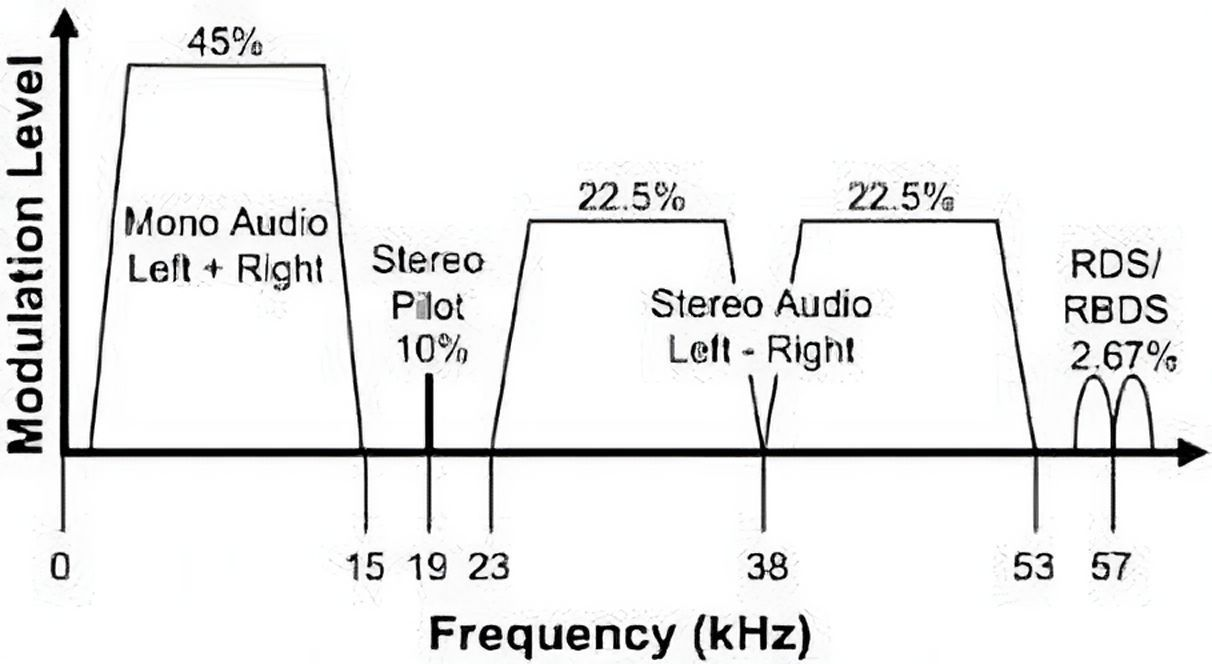
\includegraphics[width = 0.6\linewidth]{img/mpx_signal_spectrum.jpeg}
    \caption{Espectro da mensagem de um sinal FM stereo.}
    \label{fig:stereo_spectrum}
\end{figure}

Após a recuperaç\~ao dos sinais $m_1(t)$ e $m_2(t)$, obtém-se trivialmente os sinais desejados, $L$ e $R$, através do processo de \textit{dematrixing}:

\begin{equation*}
  \left\{\begin{array}{@{}l@{}}
    m_1(t)+m_2(t)=2L\\
    m_1(t)-m_2(t)=2R
  \end{array}\right.\,.
\end{equation*}

Apresenta-se então, na \hyperref[fig:desmodulador FM stereo]{Fig. 2} um esquema simplificado do processo de desmultiplexaç\~ao, posterior à desmodulaç\~ao do sinal FM.

\begin{figure}[H]
    \centering
    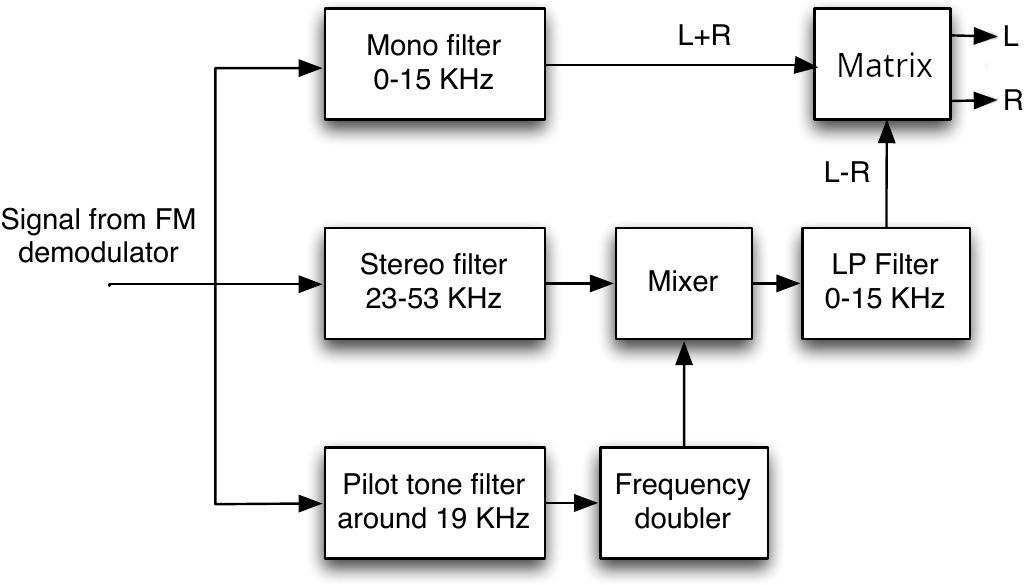
\includegraphics[width = 0.6\linewidth]{img/stereo_demultiplexing.jpeg}
    \caption{Modelo simplificado do descodificador stereo.}
    \label{fig:desmodulador FM stereo}
\end{figure}
%1
%1
%=============================--B--=============================%
\newpage
\subsection{Desmodulaç\~ao de um sinal FM}
Na secção anterior partimos do princípio que já temos o sinal m(t), mas na transmiss\~ao de um sinal FM é realizado uma modulação da mensagem, tal que o sinal que o recetor recebe é o seguinte:

\begin{equation*}
    x_{FM}(t)=A_c \cos{(2\pi f_c t + 2 \pi k_f  \int_{-\infty}^{t} m(\lambda) \,d\lambda)}
\end{equation*}

É então nossa tarefa recuperar a mensagem m(t) a partir do sinal $x_{FM}(t)$. Para tal existem 2 opções:

\vspace{0.5em}
\textbf{Opção 1:}
Uma vez que a mensagem está na frequência do cosseno, a opção mais intuitiva seria derivar o sinal $x_{FM}(t)$ e utilizar um detetor de envolvente.

\begin{equation*}
    \frac{1}{2\pi} \frac{\partial x_{FM}(t)}{\partial x} =
    A_c (f_c + k_f m(t))\cos{\left(2\pi f_c t + 2 \pi k_f  \int_{-\infty}^{t} m(\lambda) \,d\lambda + \frac{\pi}{2}\right)}
\end{equation*}

Uma vez que a amplitude do sinal resultante segue o andamento de m(t), pode-se utilizar um detetor de envolvente para recuperar a mensagem.

\vspace{1.5em}

\textbf{Opção 2:}

Utilizar um desmodulador em quadratura. 
Este desmodulador começa com um misturador que faz a heterodinagem do sinal, "arrastando-o" de modo a ficar centrado em $f_I$ em vez de $f_c$, visto que os filtros posteriores estão centrados nessa frequência.

De seguida através do produto por um cosseno e um sinal retira a componente em fase ($x_I(t)$) e em quadratura ($x_Q(t)$) do sinal $x_{FM}(t)$. Obtendo-se o seguinte sinal:

\begin{equation*}
    x(t)=x_I(t)\cos{(2 \pi f_I t)} - x_Q(t)\sin{(2 \pi f_I t)}
\end{equation*}

em que:

\begin{equation*}
  \left\{\begin{array}{@{}l@{}}
    x_I(t)= A_x \cos{(2 \pi k_f  \int_{-\infty}^{t} m(\lambda) \,d\lambda)}\\
    x_Q(t)= A_x \sin{(2 \pi k_f  \int_{-\infty}^{t} m(\lambda) \,d\lambda)}
  \end{array}\right.\,.
\end{equation*}

A partir das componentes em fase e quadratura, é simples descobrir a mensagem, uma vez que:

\begin{equation*}
    \frac{1}{2\pi} \arctan{\left(\frac{x_Q(t)}{x_I(t)}\right)}= k_f  \int_{-\infty}^{t} m(\lambda) \,d\lambda
\end{equation*}

Derivando o $\arctan{}$ e organizando as parcelas, obtém-se que a mensagem é dada por:

\begin{equation*}
    \therefore m(t) = \frac{1}{2\pi k_f} \frac{\partial}{\partial x}\left[\arctan{\left(\frac{x_Q(t)}{x_I(t)}\right)}\right]
\end{equation*}

    %=============================--A--=============================%
\newpage
\section{Peculiaridades}
\label{sec:peculiaridades}
De modo a manter a discussão o mais sucinta possível, serão abordados nesta secção conceitos \textbf{fulcrais} da implementação que não serão mencionados posteriormente, por questões de brevidade. Salienta-se a necessidade primordial de expor estes conceitos antes da análise do esquema desenvolvido. 
%1
%1
%=============================--B--=============================%
\subsection{1. Transition width}
\label{subsec:transition-width}
\textbf{Definição:} diferença entre a frequência em que a \textit{stopband} começa (aproximadamente, por volta dos $-60$ dB) e a frequência em que o sinal começa a ser rejeitado (i.e., quando a \textit{passband} termina; na periferia dos $-6$ dB), relativamente às frequências de corte dos filtros.

%\iffalse
\begin{figure}[H]
    \centering
    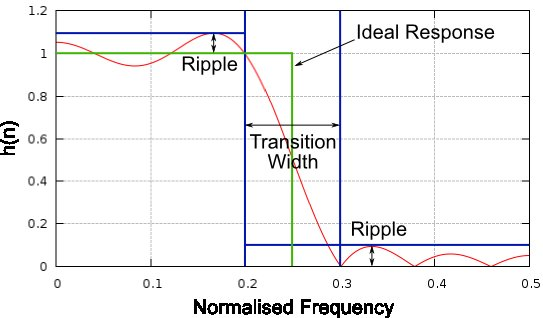
\includegraphics[width = 0.7\linewidth]{img/transition-width.png}
    \caption{Exemplo da representação da \textit{transition width} de um filtro de processamento de sinal.}
    \label{fig:transition-width}
\end{figure}
%\fi

Na elaboração do laboratório, com o uso do \textit{software} GNU Radio, foram somente utilizados filtros FIR (\textit{finite impulse response}), que apresentam uma relação entre a \hyperref[subsec:transition-width]{subsecção em discussão} e a \hyperref[subsec:delay]{seguinte}:

% https://lists.gnu.org/archive/html/discuss-gnuradio/2017-11/msg00018.html
\textit{"(...) If you use a FIR filter and use a small transition width, processing speed of the program will degrade, as more filter taps are needed. If you use a large transition width, the speed of the program improves (less taps are needed), but you have to deal with the lousy frequency response of the filter. (...)"}\cite{fwd:transitionwidth}

Fator delimitado com base nestes \textit{trade-offs} verificados empiricamente.
\newline\break
\noindent\fcolorbox{black}{white}{%
    \minipage[t]{\dimexpr\linewidth-2\fboxsep-2\fboxrule\relax}
        \textbf{Observações} $\rightarrow$ Para valores ínfimos deste parâmetro, verificou-se uma perda de informação indesejável do sinal. No espectro oposto, para elevados valores de transição, foi constatada uma captação de informação não solicitada (apesar de atenuada; vide a \hyperref[fig:transition-width]{imagem acima}) e maior prevalência de ruído.
    \endminipage}
\newline\break
Foi admitida uma \textit{transition width} de $1$ kHz na maioria dos filtros implementados, nomeadamente do \hyperref[subsec:mod3]{módulo 3} (\textit{trade-off} entre delay e ruído, como veremos \hyperref[subsec:delay]{em seguida}), com exceção dos filtros passa-baixo finais com uma largura de transição diminuta de $200$ Hz (a motivação para esta modificação foi a aniquilação de perturbações sonóras, derivadas do ruído, experienciadas).
%2
%2
%=============================--C--=============================%
\subsection{2. Delay}
\label{subsec:delay}
\textbf{Definição:} denominamos por \textit{group delay} o atraso em número inteiro de amostras, incutido pela utilização única, ao longo do projeto, de filtros do tipo \textit{"Decimating FIR filter"}, com resposta em fase linear. \\ \textit{Group delay}\cite{jayesparmarja} $\delequal K = (N-1)/2$, em que $N$ representa o número de \textit{taps} do filtro. Para obter o atraso temporal, naturalmente se deduz que: \\ \textit{Time delay}\cite{jayesparmarja} $\delequal K = (N-1)/2\text{F}_\text{S}$, onde $\text{F}_\text{S}$ denomina a frequência de amostragem (\textit{sample rate}).
\newline\break
\noindent\fcolorbox{black}{white}{%
    \minipage[t]{\dimexpr\linewidth-2\fboxsep-2\fboxrule\relax}
        \textbf{Observações} $\rightarrow$ Com o aumento da \textit{sample rate} verifica-se uma diminuição do \textit{delay} temporal.
        O \textit{group delay} aumenta linearmente com o número de \textit{taps} do filtro.
    \endminipage}
\newline\break

Dado que o \textit{source code} do \textit{software} GNU Radio utilizado se encontra disponível (distribuído sobre os termos da licença GPL e \textit{copyrighted} pela Free Software Foundation), foi efetuada uma análise sucinta que se traduziu em ilações bastante curiosas.

\begin{lstlisting}[caption=\textit{Source code}: \color{white}{\underline{https://github.com/gnuradio/gnuradio/blob/master/gr-filter/lib/firdes.cc}}, frame=tlrb]{saucecode}
int firdes::compute_ntaps_windes(
    double sampling_freq,
    double transition_width, // this is frequency, not relative frequency
    double attenuation_dB)
{
    // Based on formula from Multirate Signal Processing for
    // Communications Systems, fredric j harris
    int ntaps = (int)(attenuation_dB * sampling_freq / (22.0 * transition_width));
    if ((ntaps & 1) == 0) // if even...
        ntaps++;          // ...make odd
    return ntaps;
}

int firdes::compute_ntaps(double sampling_freq,
                          double transition_width,
                          fft::window::win_type window_type,
                          double param)
{
    double a = fft::window::max_attenuation(window_type, param);
    int ntaps = (int)(a * sampling_freq / (22.0 * transition_width));
    if ((ntaps & 1) == 0) // if even...
        ntaps++;          // ...make odd

    return ntaps;
}
\end{lstlisting}

É diretamente observado que o número de \textit{taps} é inversamente proporcional à \textit{transition width}, i.e., uma menor \textit{transition width} traduz-se num maior \textit{delay}. Fica então corroborada a relação íntima entre \hyperref[subsec:delay]{esta subsecção} com \hyperref[subsec:transition-width]{a anterior}, como supramencionado. 

Verifica-se que para uma dada frequência de corte, uma \textit{transition width} menor, corresponde a uma \textit{roll-off slope} mais acentuada (maior ordem do filtro, no sentido familiar analógico). Pelo que o número de \textit{taps} representa a ordem do filtro. É então de fácil entendimento a degradação do tempo de processamento do programa com o incremento do número de \textit{taps}.

Outro aspecto a salientar é o facto do número de \textit{taps} se encontrar diretamente proporcional à \textit{sample rate}, o que reporta o melhor funcionamento dos filtros utilizados a altas frequências de amostragem.
\newline\break
\noindent\fcolorbox{black}{white}{%
    \minipage[t]{\dimexpr\linewidth-2\fboxsep-2\fboxrule\relax}
        \textbf{Observações} $\rightarrow$ Para os parâmetros projetados (\textit{transition width} e \textit{sample rate}), o \textit{delay} que compensa o atraso induzido no ramo que efetua a recuperação de $L - R$ (dado que apresenta o maior número de filtragens) é de 25 \textit{samples}. A localização escolhida e observada no \hyperref[subsec:mod1]{módulo 1} (no seguimento deste documento), leva a que as componentes $L+R$ e $L-R$ se encontrem síncronas à entrada do \hyperref[subsec:mod4]{módulo 4} que efetua o processo de \textit{dematrixing} (admitindo a calibração efetuada com os ficheiros de teste fornecidos na página da UC com este propósito: LEFT e RIGHT; esta síncronia verifica-se na fase e na oposição de fase destas duas componentes ($L+R$ e $L-R$), para os casos respectivos, como aparente nas \hyperref[fig:multiplas]{figuras seguintes}).
    \endminipage}

\begin{figure}[ht] 
    \begin{subfigure}[b]{0.5\linewidth}
        \centering
        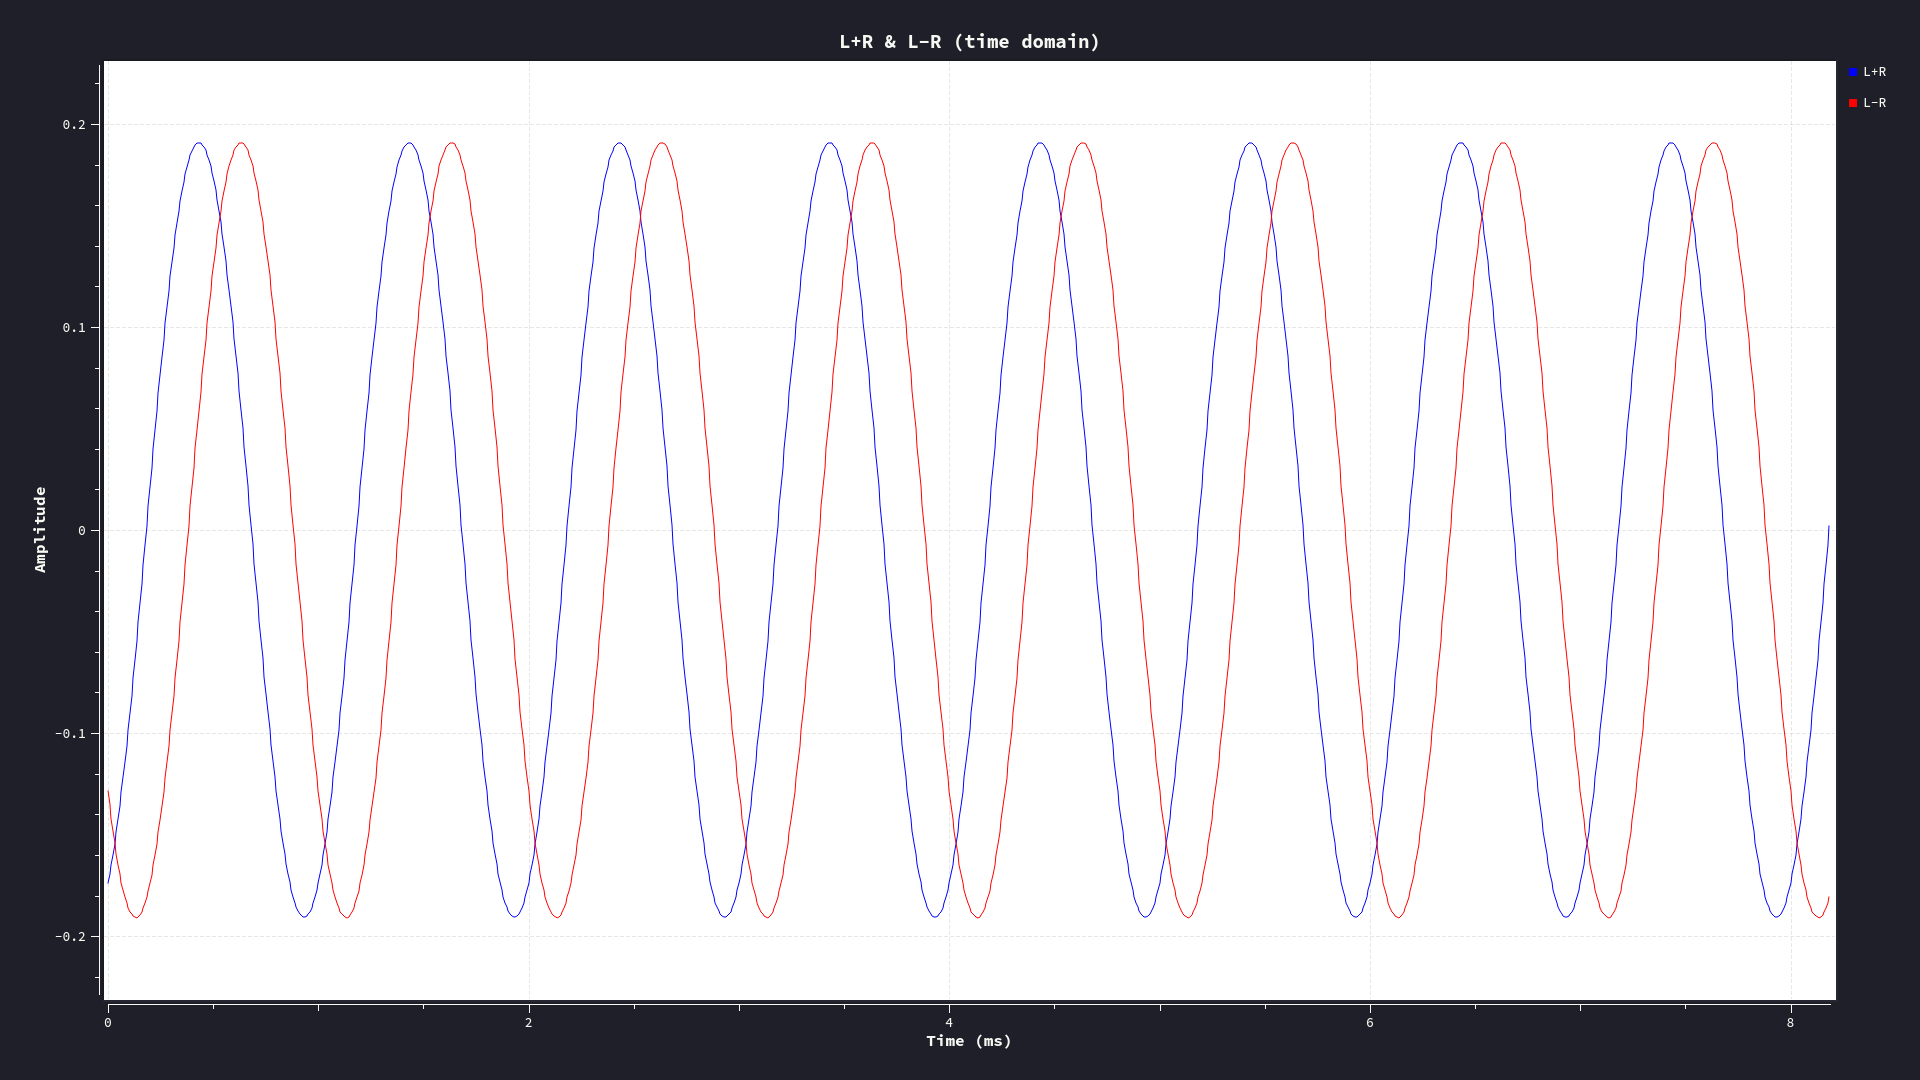
\includegraphics[width=0.9\linewidth]{img/peculiaridades/LEFT_sem_delay.png}
        \caption{LEFT: visualização de $L+R$ e $L-R$ sem \textit{delay}.} 
        \label{fig:a} 
        \vspace{4ex}
    \end{subfigure}%% 
    \begin{subfigure}[b]{0.5\linewidth}
        \centering
        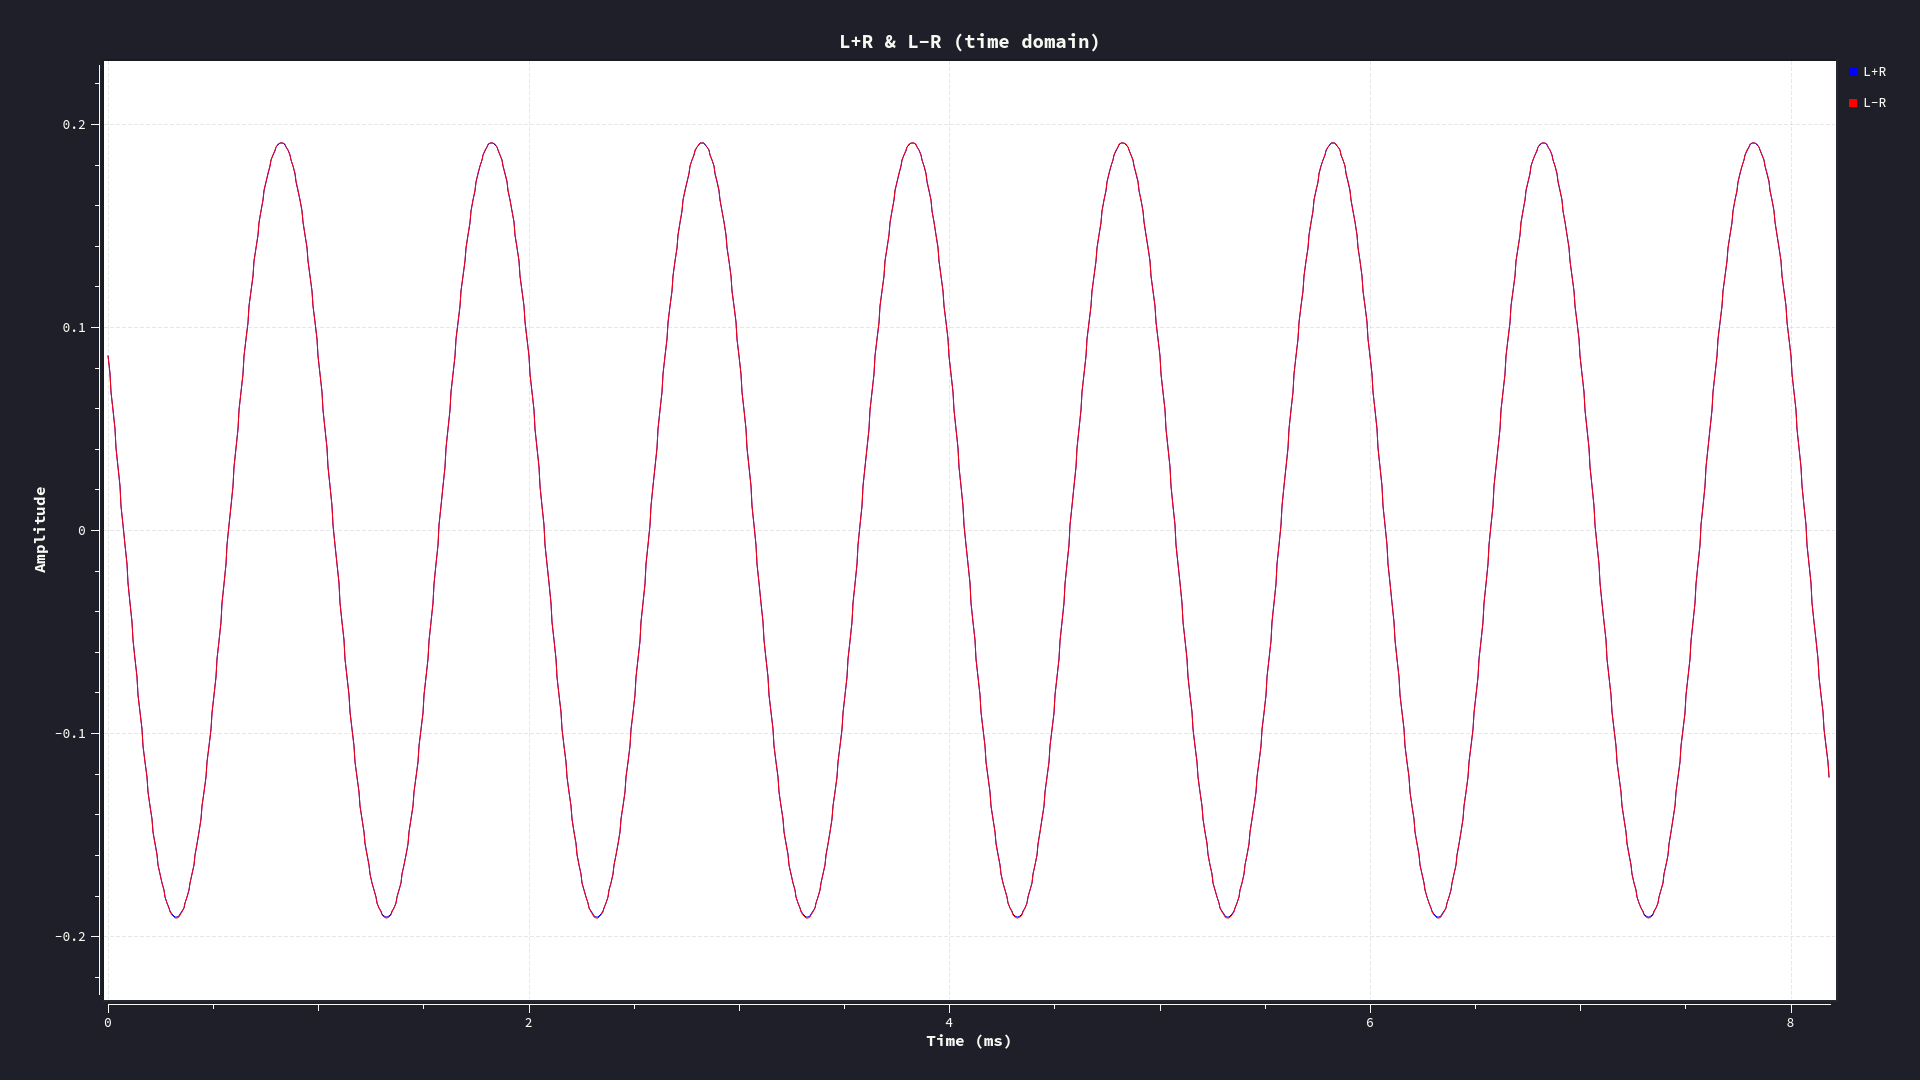
\includegraphics[width=0.9\linewidth]{img/peculiaridades/LEFT_com_delay.png} 
        \caption{LEFT: visualização de $L+R$ e $L-R$ com \textit{delay}.} 
        \label{fig:b} 
        \vspace{4ex}
    \end{subfigure} 
    \begin{subfigure}[b]{0.5\linewidth}
        \centering
        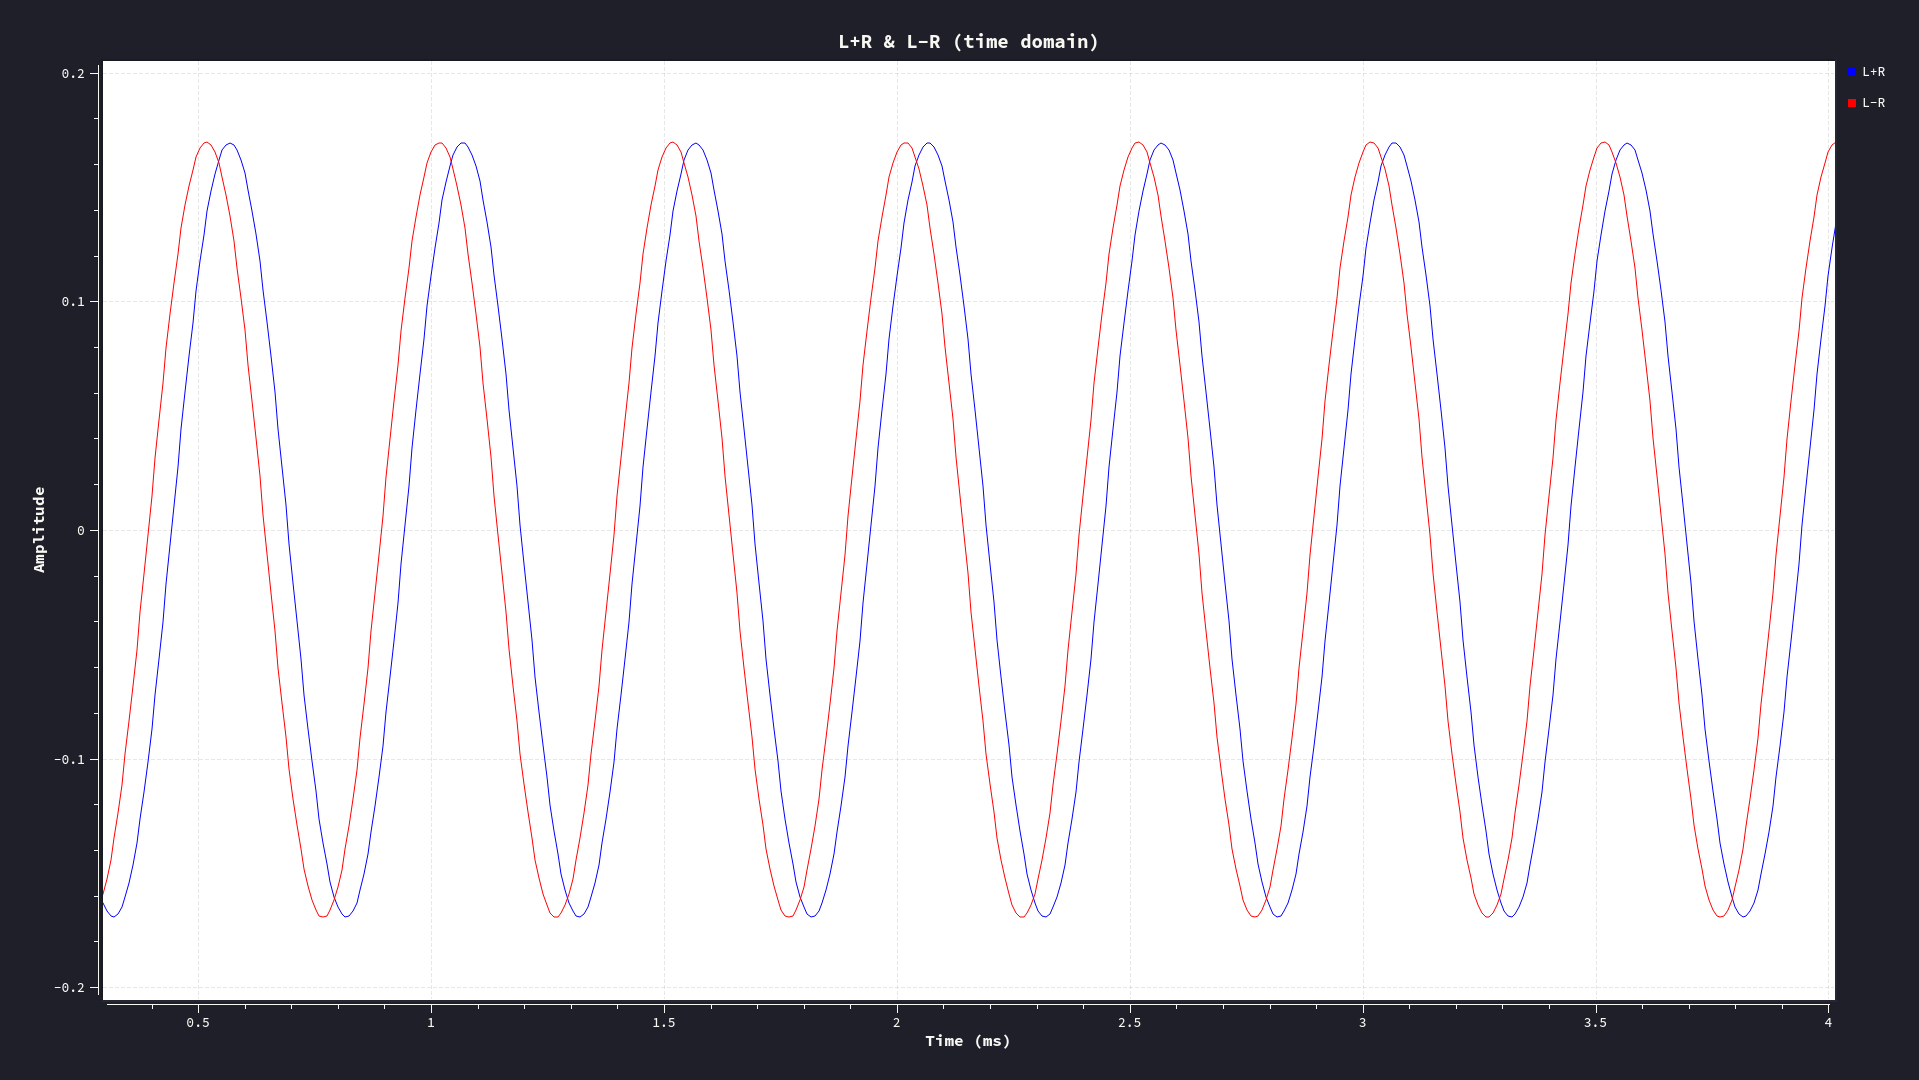
\includegraphics[width=0.9\linewidth]{img/peculiaridades/RIGHT_sem_delay.png}
        \caption{RIGHT: visualização de $L+R$ e $L-R$ sem \textit{delay}.} 
        \label{fig:c} 
        %%\vspace{4ex}
    \end{subfigure}%% 
    \begin{subfigure}[b]{0.5\linewidth}
        \centering
        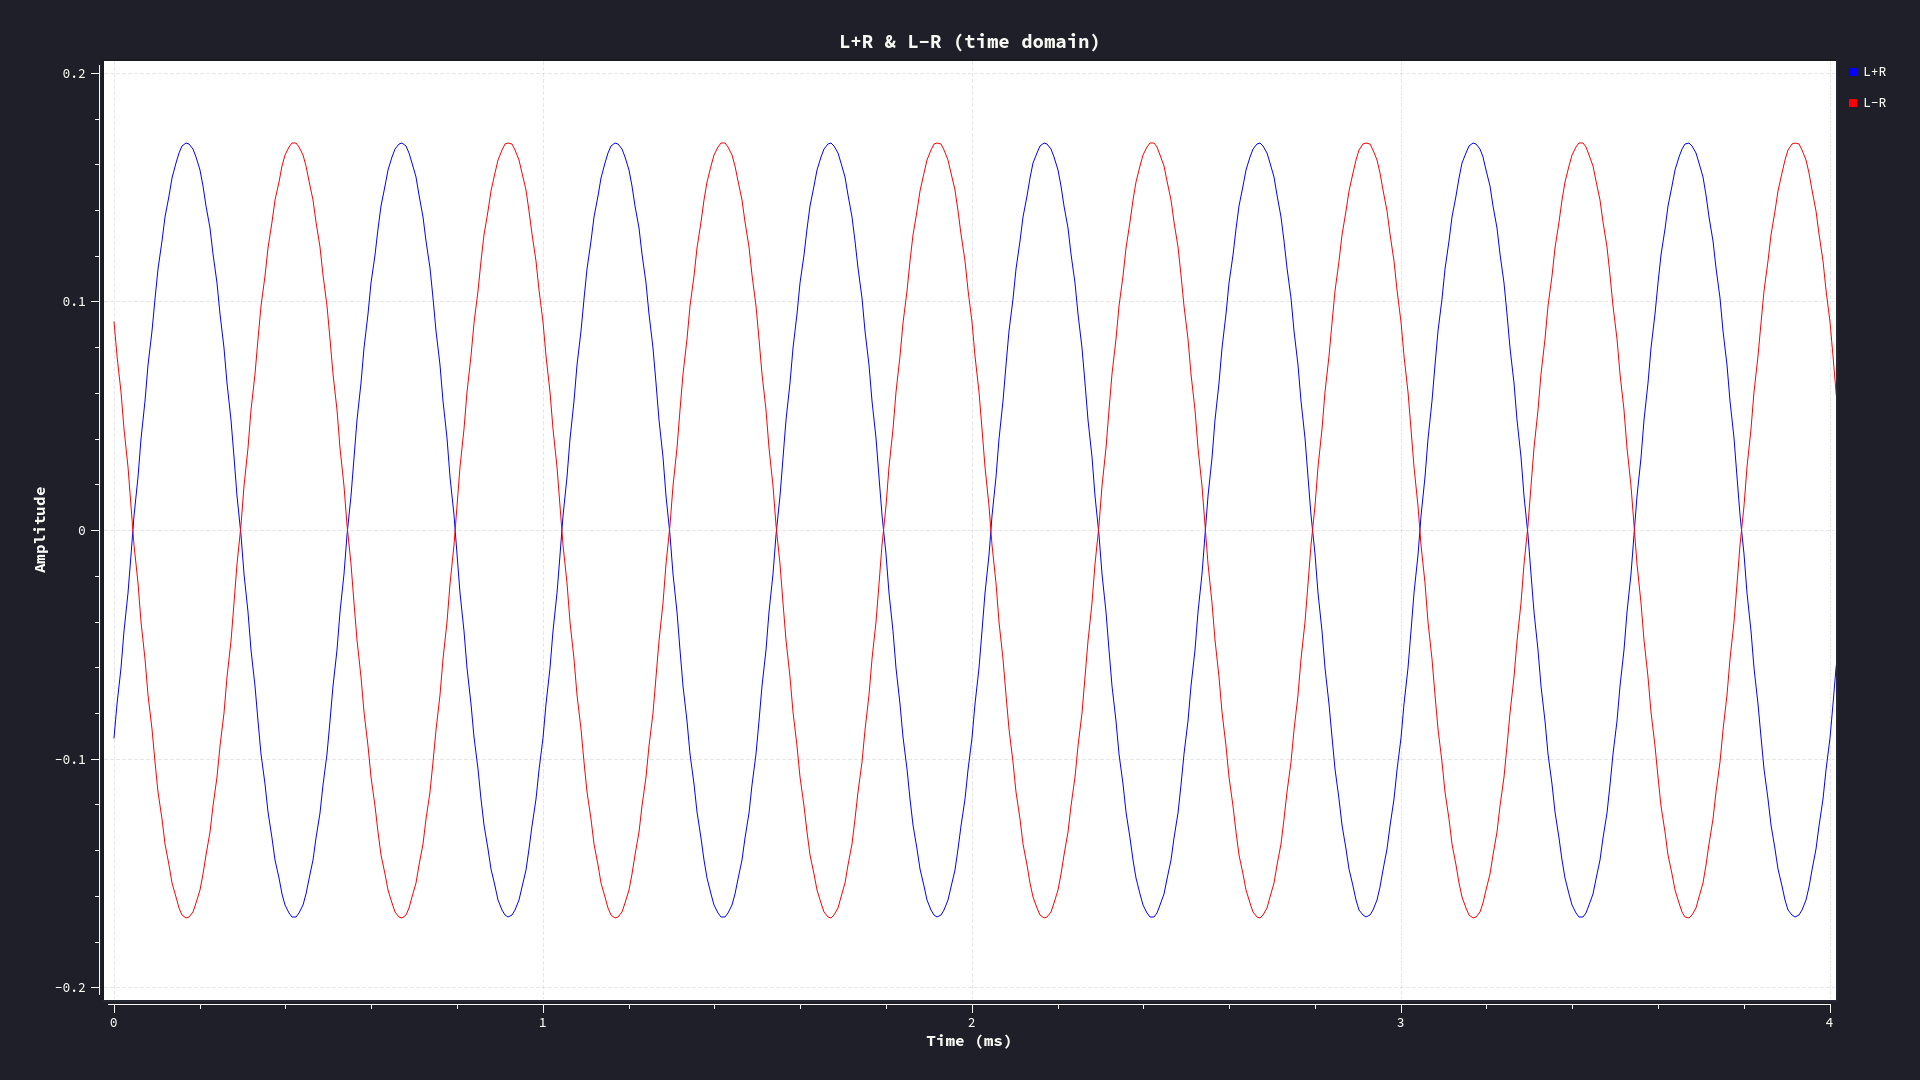
\includegraphics[width=0.9\linewidth]{img/peculiaridades/RIGHT_com_delay.png} 
        \caption{RIGHT: visualização de $L+R$ e $L-R$ com \textit{delay}.} 
        \label{fig:d} 
        %%\vspace{4ex}
    \end{subfigure} 
    \caption{Efeitos da calibração com o bloco de \textit{delay} no final do ramo que recupera $L+R$.}
    \label{fig:multiplas}
\end{figure}
%3
%3
%=============================--D--=============================%
\subsection{3. Filtros de de-ênfase}

%\iffalse
\begin{figure}[H]
    \centering
    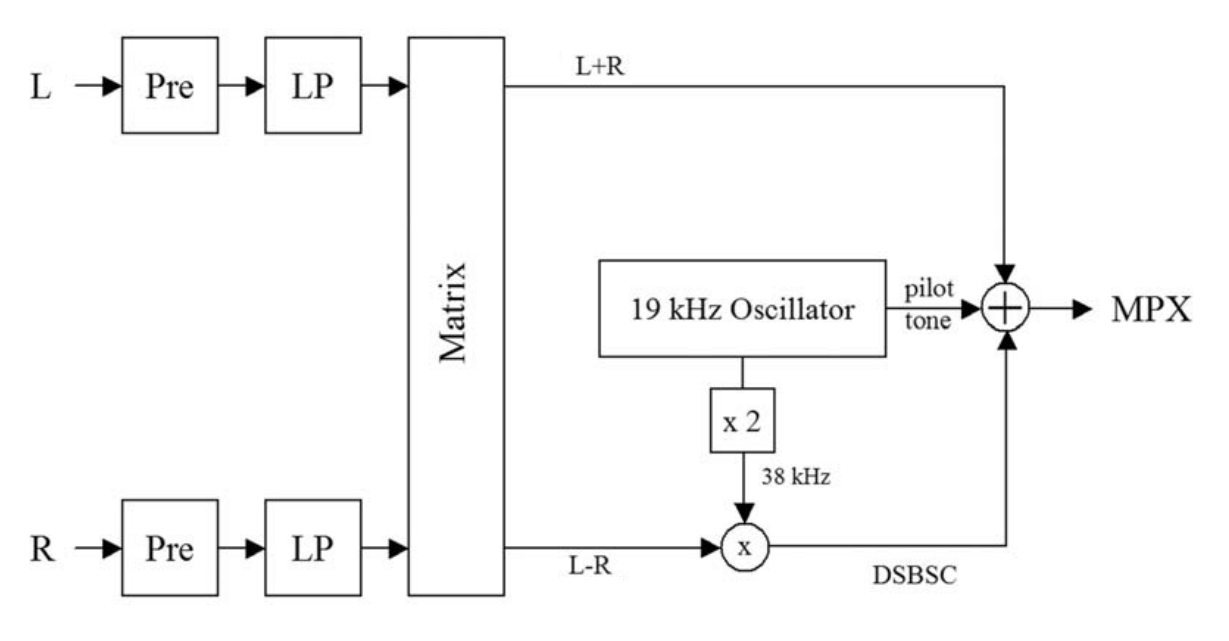
\includegraphics[width = 0.7\linewidth]{img/peculiaridades/encoder_stereo.png}
    \caption{Codificador stereo com filtros de pré-ênfase (Pre) e filtros passa-baixo (LP).}
    \label{fig:stereo_encoder}
\end{figure}
%\fi

No processo de codificação da mensagem, exposto na \hyperref[fig:stereo_encoder]{Fig. 5}, os sinais $L$ e $R$ são sujeitos a filtros de pré-ênfase com o intuito delineado na seguinte citação:

\textit{"Pre-emphasis (giving High frequencies a boost) is applied to both channels before the multiplexing process. A corresponding de-emphasis is applied at the receiver. The idea of this is to lift the high frequency signal some so that in the receiver you can reduce the high frequency ALONG WITH some of the hiss from the receiver. In Australia [NOTA: o mesmo para a Europa\cite{transmission_standards_for_fm_sound_broadcasting_at_vhf}] we use a $50\ \mu$s time constant network for pre-emphasis, in USA they use $75\ \mu$s."}\cite{anintroductiontofmmpx}

\vspace{1.0em}
Tendo em conta o supracitado e a seguinte \hyperref[fig:bb]{Fig. 6 (b)}, é trivialmente deduzida a localização dos filtros de de-ênfase (\hyperref[fig:aa]{Fig. 6 (a)}).

\begin{figure}[ht] 
    \begin{subfigure}[b]{0.5\linewidth}
        \centering
        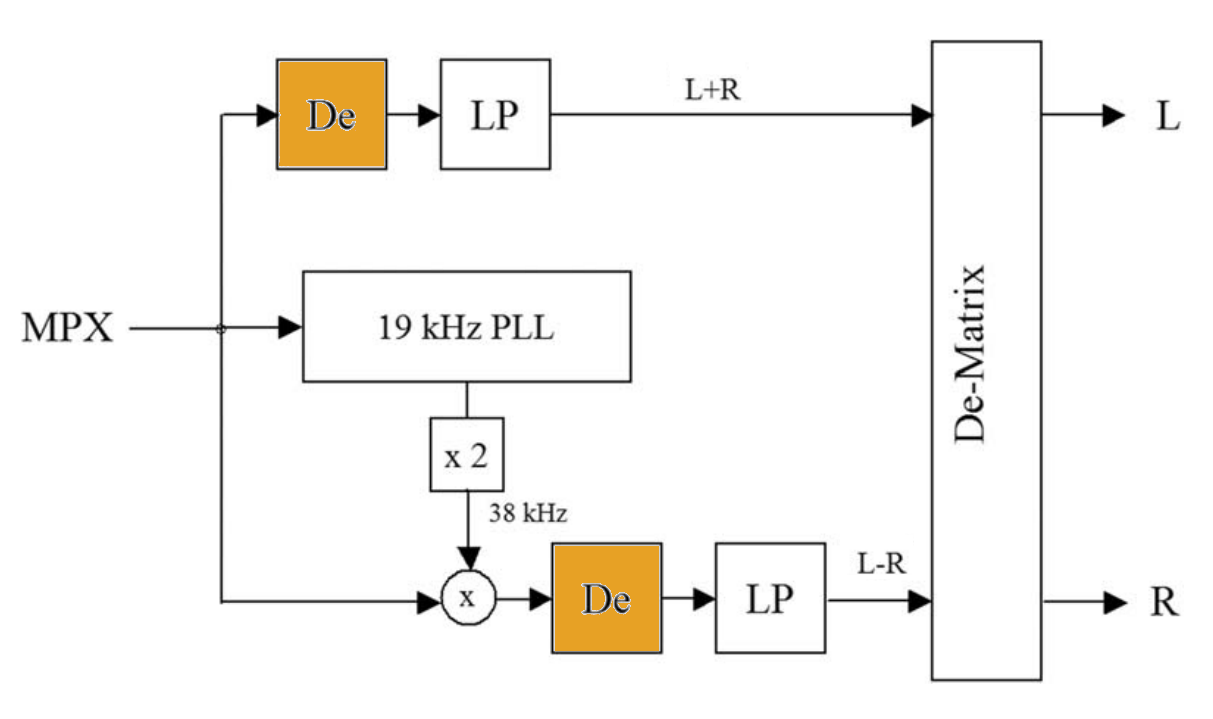
\includegraphics[width=0.90\linewidth]{img/peculiaridades/decoder_stereo.png}
        \caption{Descodificador stereo com \textcolor{orange}{filtros de de-ênfase (De)} \\ e filtros passa-baixo (LP).} 
        \label{fig:aa} 
        %\vspace{4ex}
    \end{subfigure}%% 
    \begin{subfigure}[b]{0.5\linewidth}
        \centering
        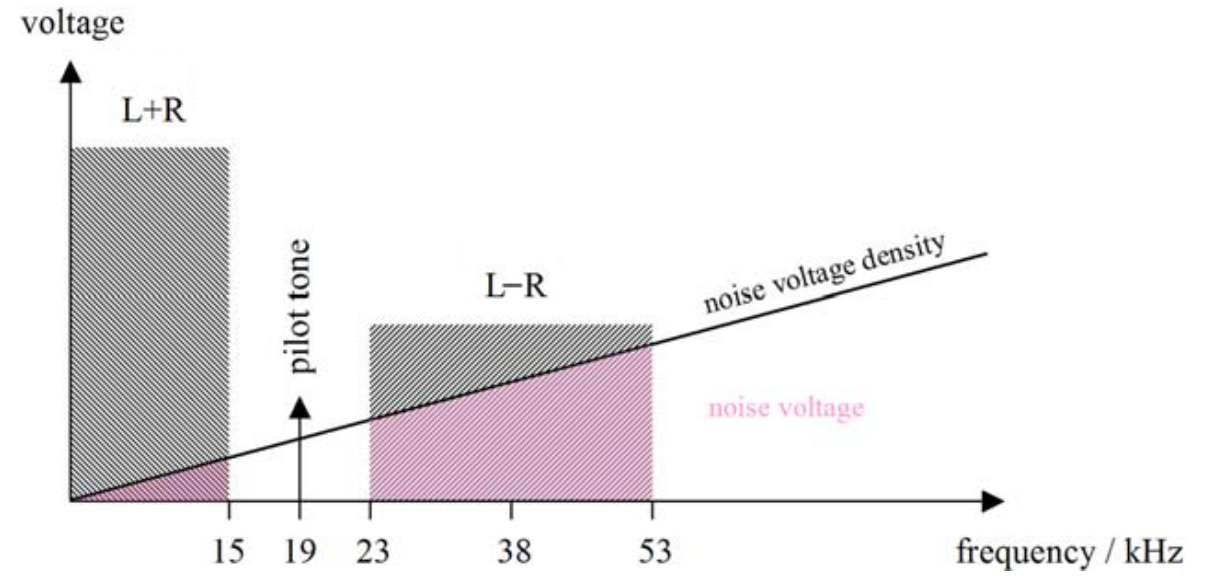
\includegraphics[width=0.90\linewidth]{img/peculiaridades/noise.png} 
        \caption{\textit{Noise voltage density} e \textit{\textcolor{pink}{noise voltage}}, sinais $L+R$ \\ e $L-R$.} 
        \label{fig:bb} 
        %\vspace{4ex}
    \end{subfigure} 
    \caption{De-ênfase.}
    \label{fig:multiplas2}
\end{figure}

O processo de de-ênfase efetua-se nos módulos \hyperref[subsec:mod2]{2} e \hyperref[subsec:mod3]{3} (antes dos filtros passa-baixo com $f_c = 15$ kHz), de modo a mitigar a \textit{noise voltage} das componentes $L+R$ e $L-R$. O resultado final traduz-se numa maior qualidade sonora à saída do \textit{dematrixer} (\hyperref[subsec:mod4]{módulo 4}).
\newline\break
\noindent\fcolorbox{black}{white}{%
    \minipage[t]{\dimexpr\linewidth-2\fboxsep-2\fboxrule\relax}
        \textbf{Observações} $\rightarrow$ A não utilização destes filtros supramencionados (no caso do sinal de teste IQ e transmissões rádio captadas pelo RTL-SDR), manifestou-se na presença audível de "som de estática" que deteriorou a qualidade sónora (o \textit{signal-to-noise ratio} é diminuído, perceptivelmente, com o aumento do ruído de fundo). A disposição destes blocos antes do "Audio Sink" resultou na redução de ruído de fundo, no entanto, este verificou-se \textit{muffled} (não ideal). A localização explicitada na \hyperref[fig:aa]{Fig. 6 (a)}, mostrou-se incrivelmente eficiente na redução do ruído audível, e não comprometeu a fidedignidade sonora.
    \endminipage}

    \newpage
\renewcommand{\thefigure}{M\arabic{figure}}
\renewcommand{\thetable}{M\arabic{table}}
\setcounter{figure}{0}
\section{Implementação}
%=============================--A--=============================%
\subsection{Módulo 1 $\pmb \mapsto$ Desmodulaç\~ao}
\label{subsec:mod1}

%\iffalse
\begin{figure}[H]
    \centering
    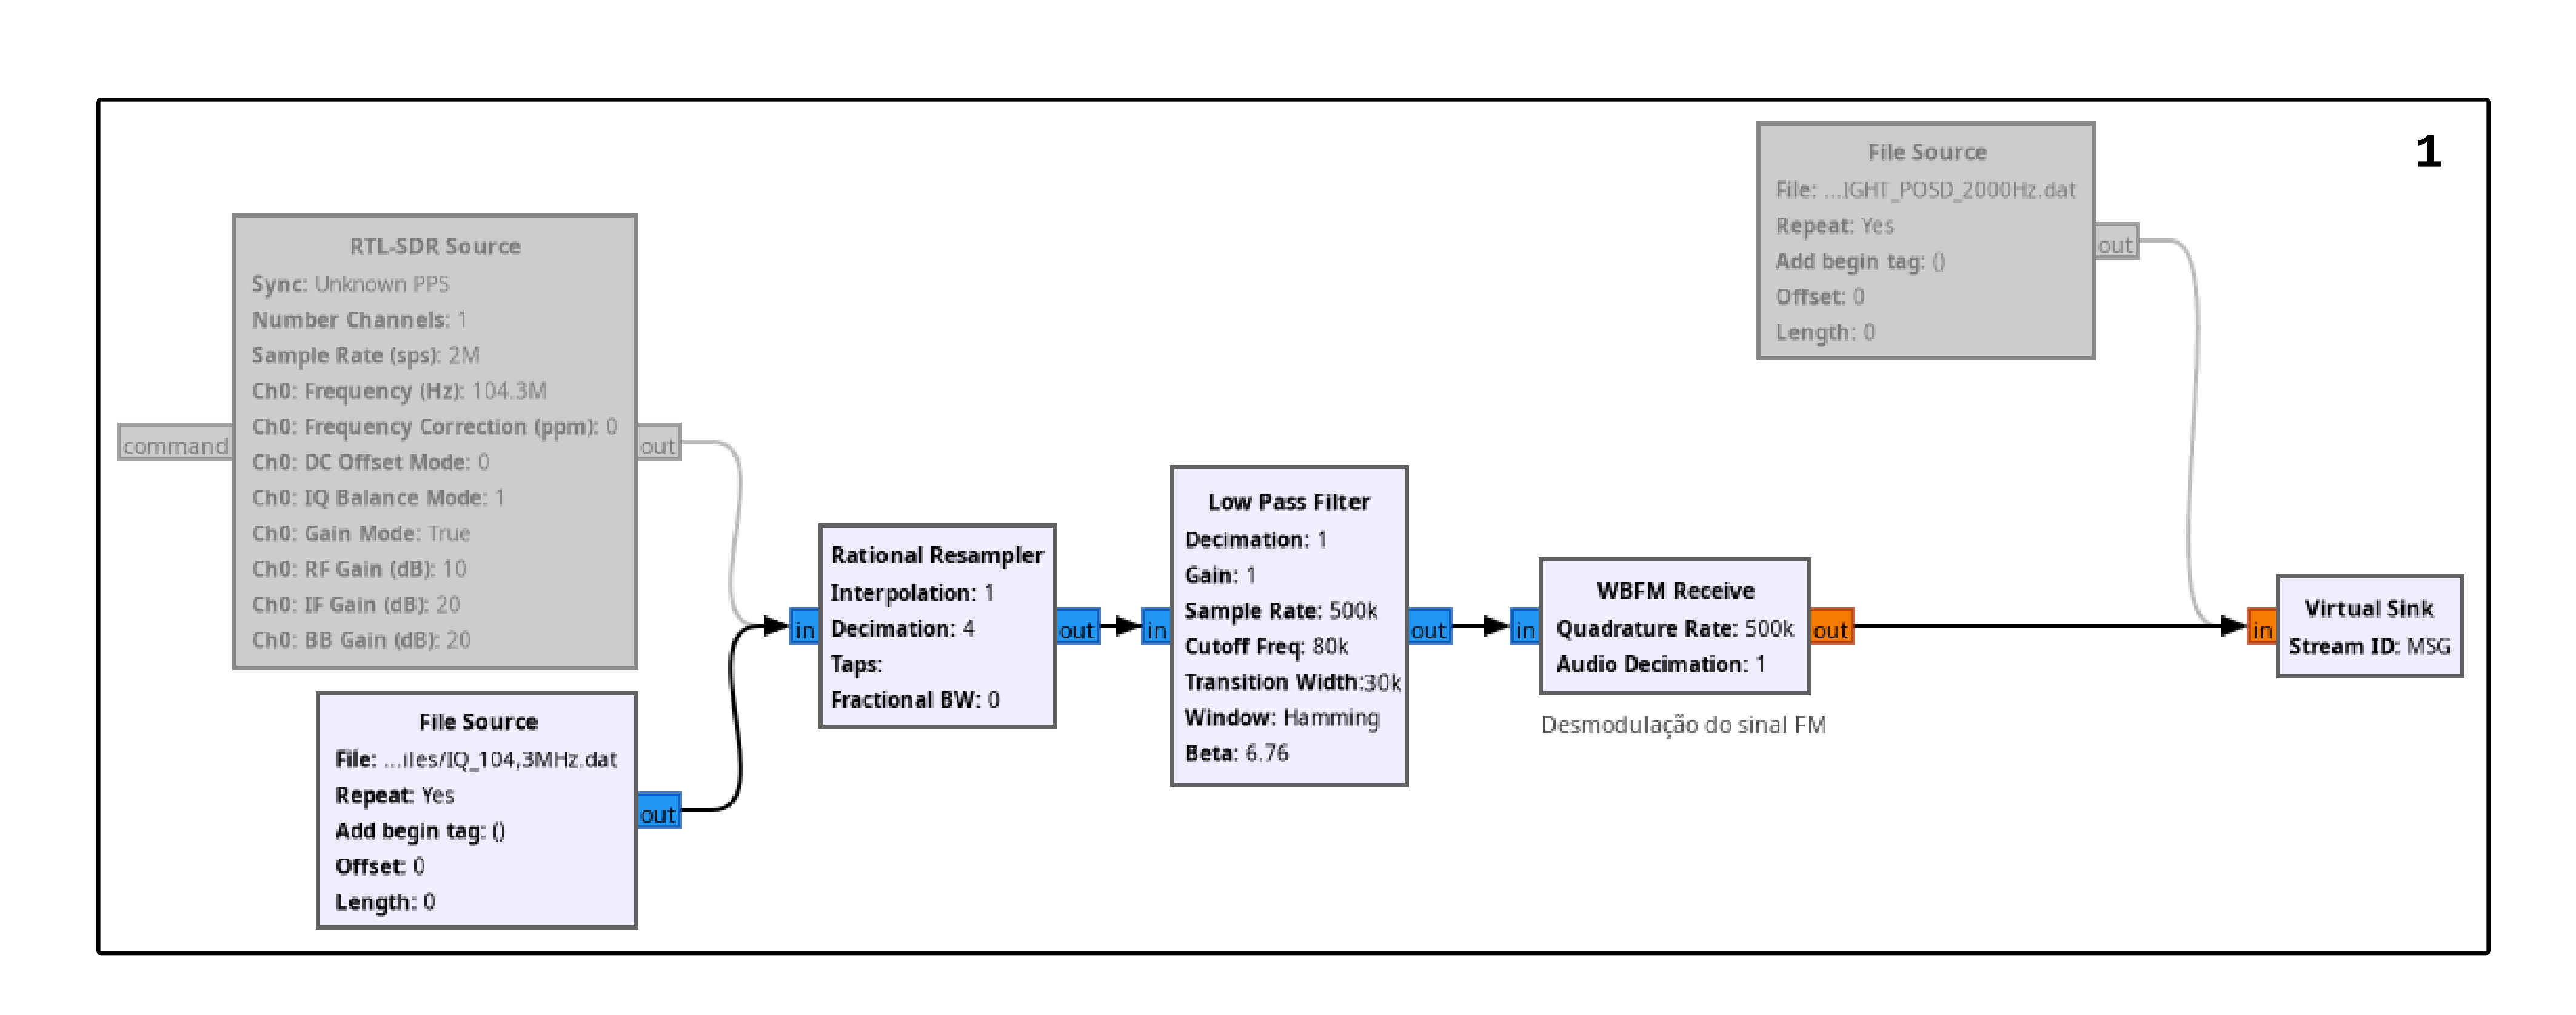
\includegraphics[width = 1\linewidth]{img/mods/modulo1.png}
    \caption{Processo de obtenção do sinal mensagem multiplexado $m(t)$.}
    \label{fig:modulo1}
\end{figure}
%\fi

Os sinais recebidos pela antena ou extraído dos ficheiros de testes (associado ao bloco "RTL-SDR Source" e "File Source" respetivamente), são sinais FM, logo no formato:

\begin{equation*}
    x_{FM}(t)=A_c \cos{(2\pi f_c t + 2 \pi k_f  \int_{-\infty}^{t} m(\lambda) \,d\lambda)}
\end{equation*}
 
Tal como já mencionado, na introdução, para desmodular um sinal FM utiliza-se um desmodulador em quadratura, que se encontra no bloco "WBFM Receive". Este também contém um filtro de de-ênfase (para compensar a pré-ênfase do processo de modulação) e um passa-baixo, que como já referido, melhoram significativamente a qualidade do sinal.

Dado que se optou por utilizar uma frequência de amostragem de $2$ MHz, ritmo aceitável para a interface USB que vai receber as amostras do sinal, antes do sinal ser desmodulado realiza-se uma redução da frequência de amostragem por um fator de 1/4, processo este realizado no bloco de "Rational Resampler". A posterior descodificação é feita com este ritmo de amostragem de $500$ kHz.

É importante realçar que este processo de desmodulação FM é igual ao apresentado no guia laboratorial (pág. 29), uma vez que independentemente da mensagem transmitida estar num formato mono ou stereo, o processo de desmodulação FM para a obtenção da mensagem $m(t)$ é o mesmo.

No final deste modulo é colocada a mensagem multiplexada $m(t)$ numa variável de nome MSG, com auxilio do bloco "Virtual Sink".

Faz-se o reparo que os sinais de teste fornecidos LEFT e RIGHT, já se apresentam desmodulados, pelo que apenas necessitam de ser desmultiplexados para a efetuação da calibração do delay, e assim, são diretamente direcionados para o "Virtual Sink".
%=============================--A--=============================%
\subsection{Módulo 2 $\pmb \mapsto$ Recuperaç\~ao da componente mono $(L + R)$}
\label{subsec:mod2}

%\iffalse
\begin{figure}[H]
    \centering
    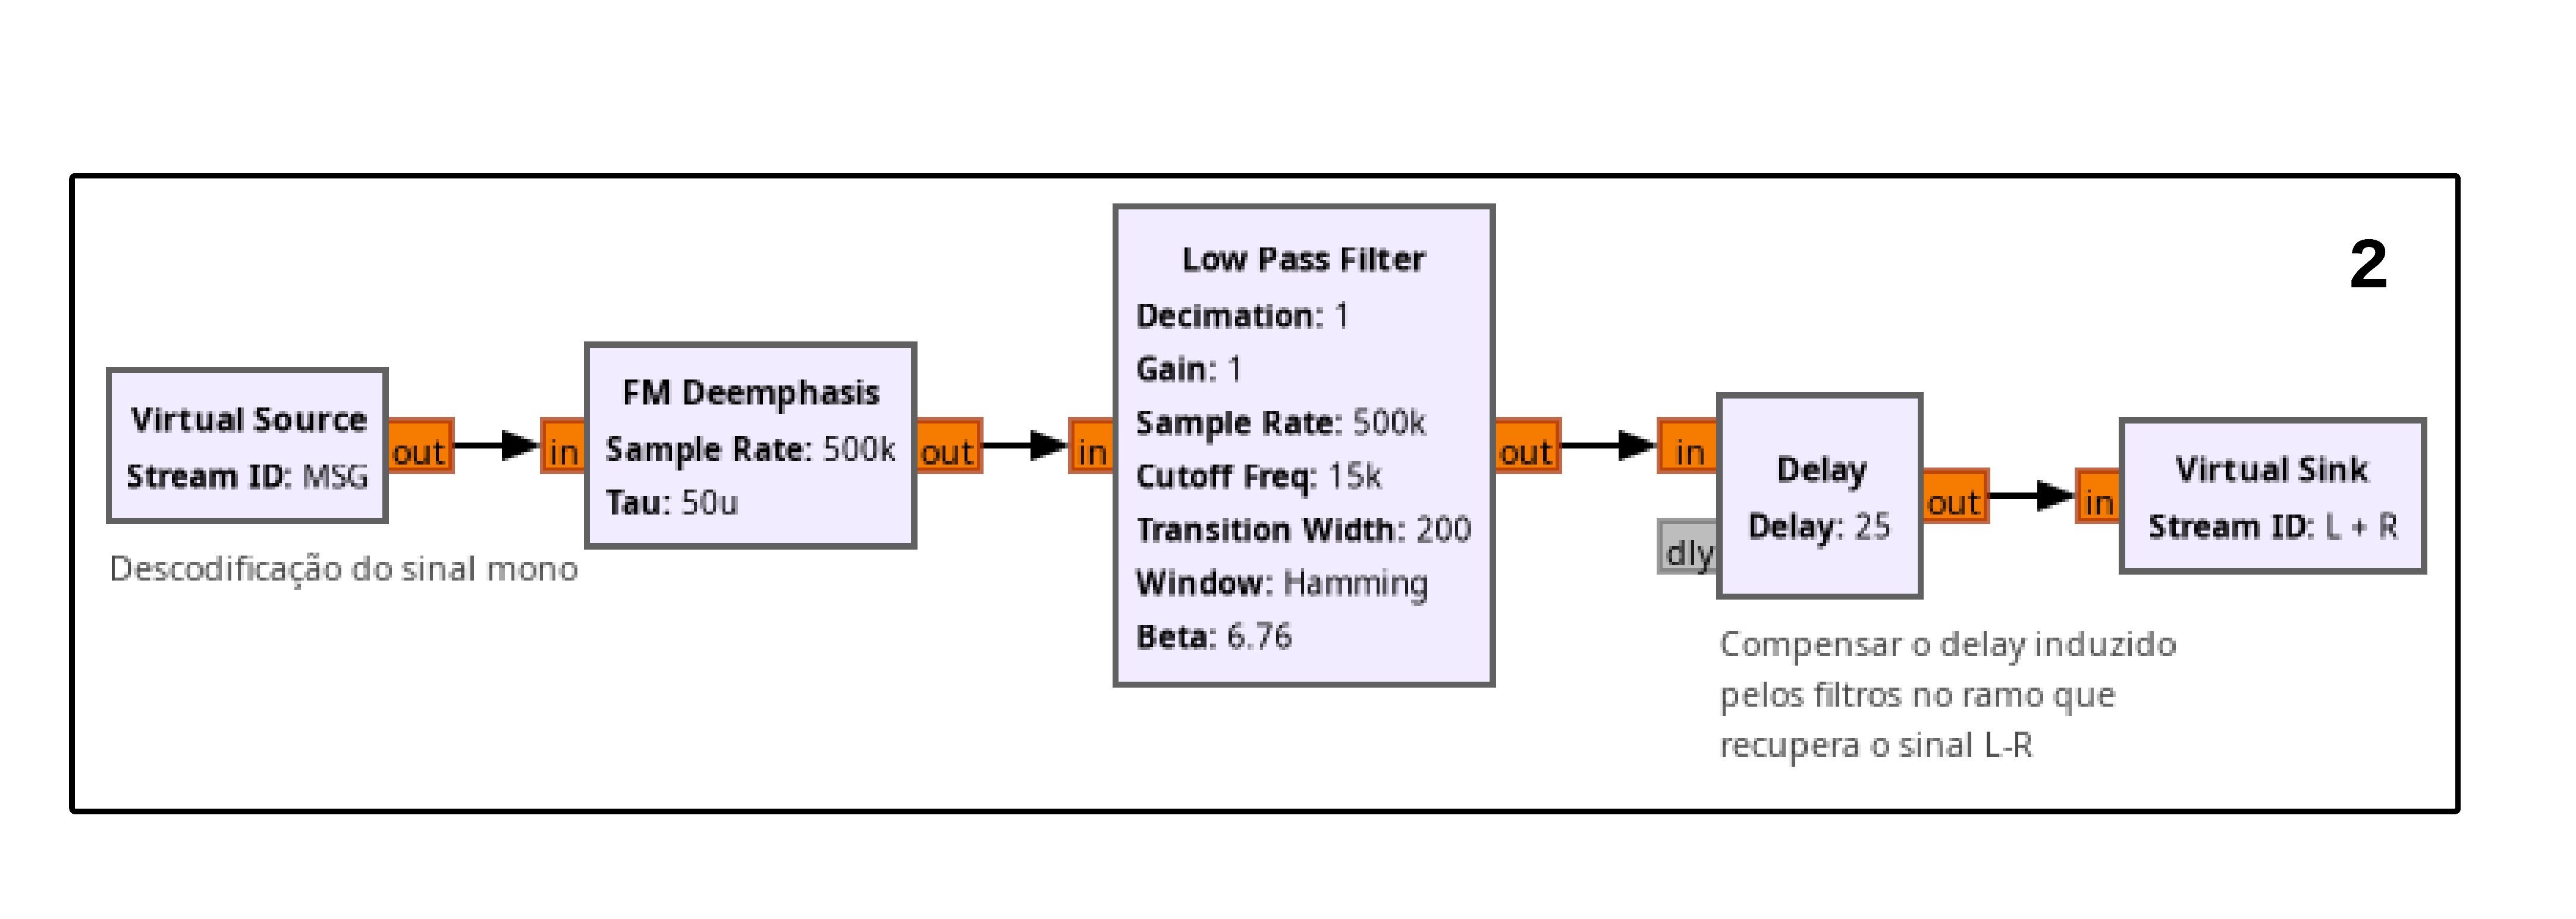
\includegraphics[width = 0.65\linewidth]{img/mods/modulo2.png}
    \caption{Recuperação da componente monofónica da mensagem.}
    \label{fig:modulo2}
\end{figure}
%\fi

De forma sucinta, o \hyperref[subsec:mod2]{módulo 2} recupera o sinal mono ($L+R$), com as correções mencionadas na secção anterior \hyperref[sec:peculiaridades]{(Peculiaridades)}, simplesmente com a aplicação de um filtro passa-baixo com $f_c = 15$ kHz, dado o formato espectral da mensagem multiplexada já abordado na introdução \hyperref[fig:stereo_spectrum]{(Fig. 1)}. 
%=============================--A--=============================%
\subsection{Módulo 3 $\pmb \mapsto$ Recuperaç\~ao da componente stereo $(L - R)$}
\label{subsec:mod3}

%\iffalse
\begin{figure}[H]
    \centering
    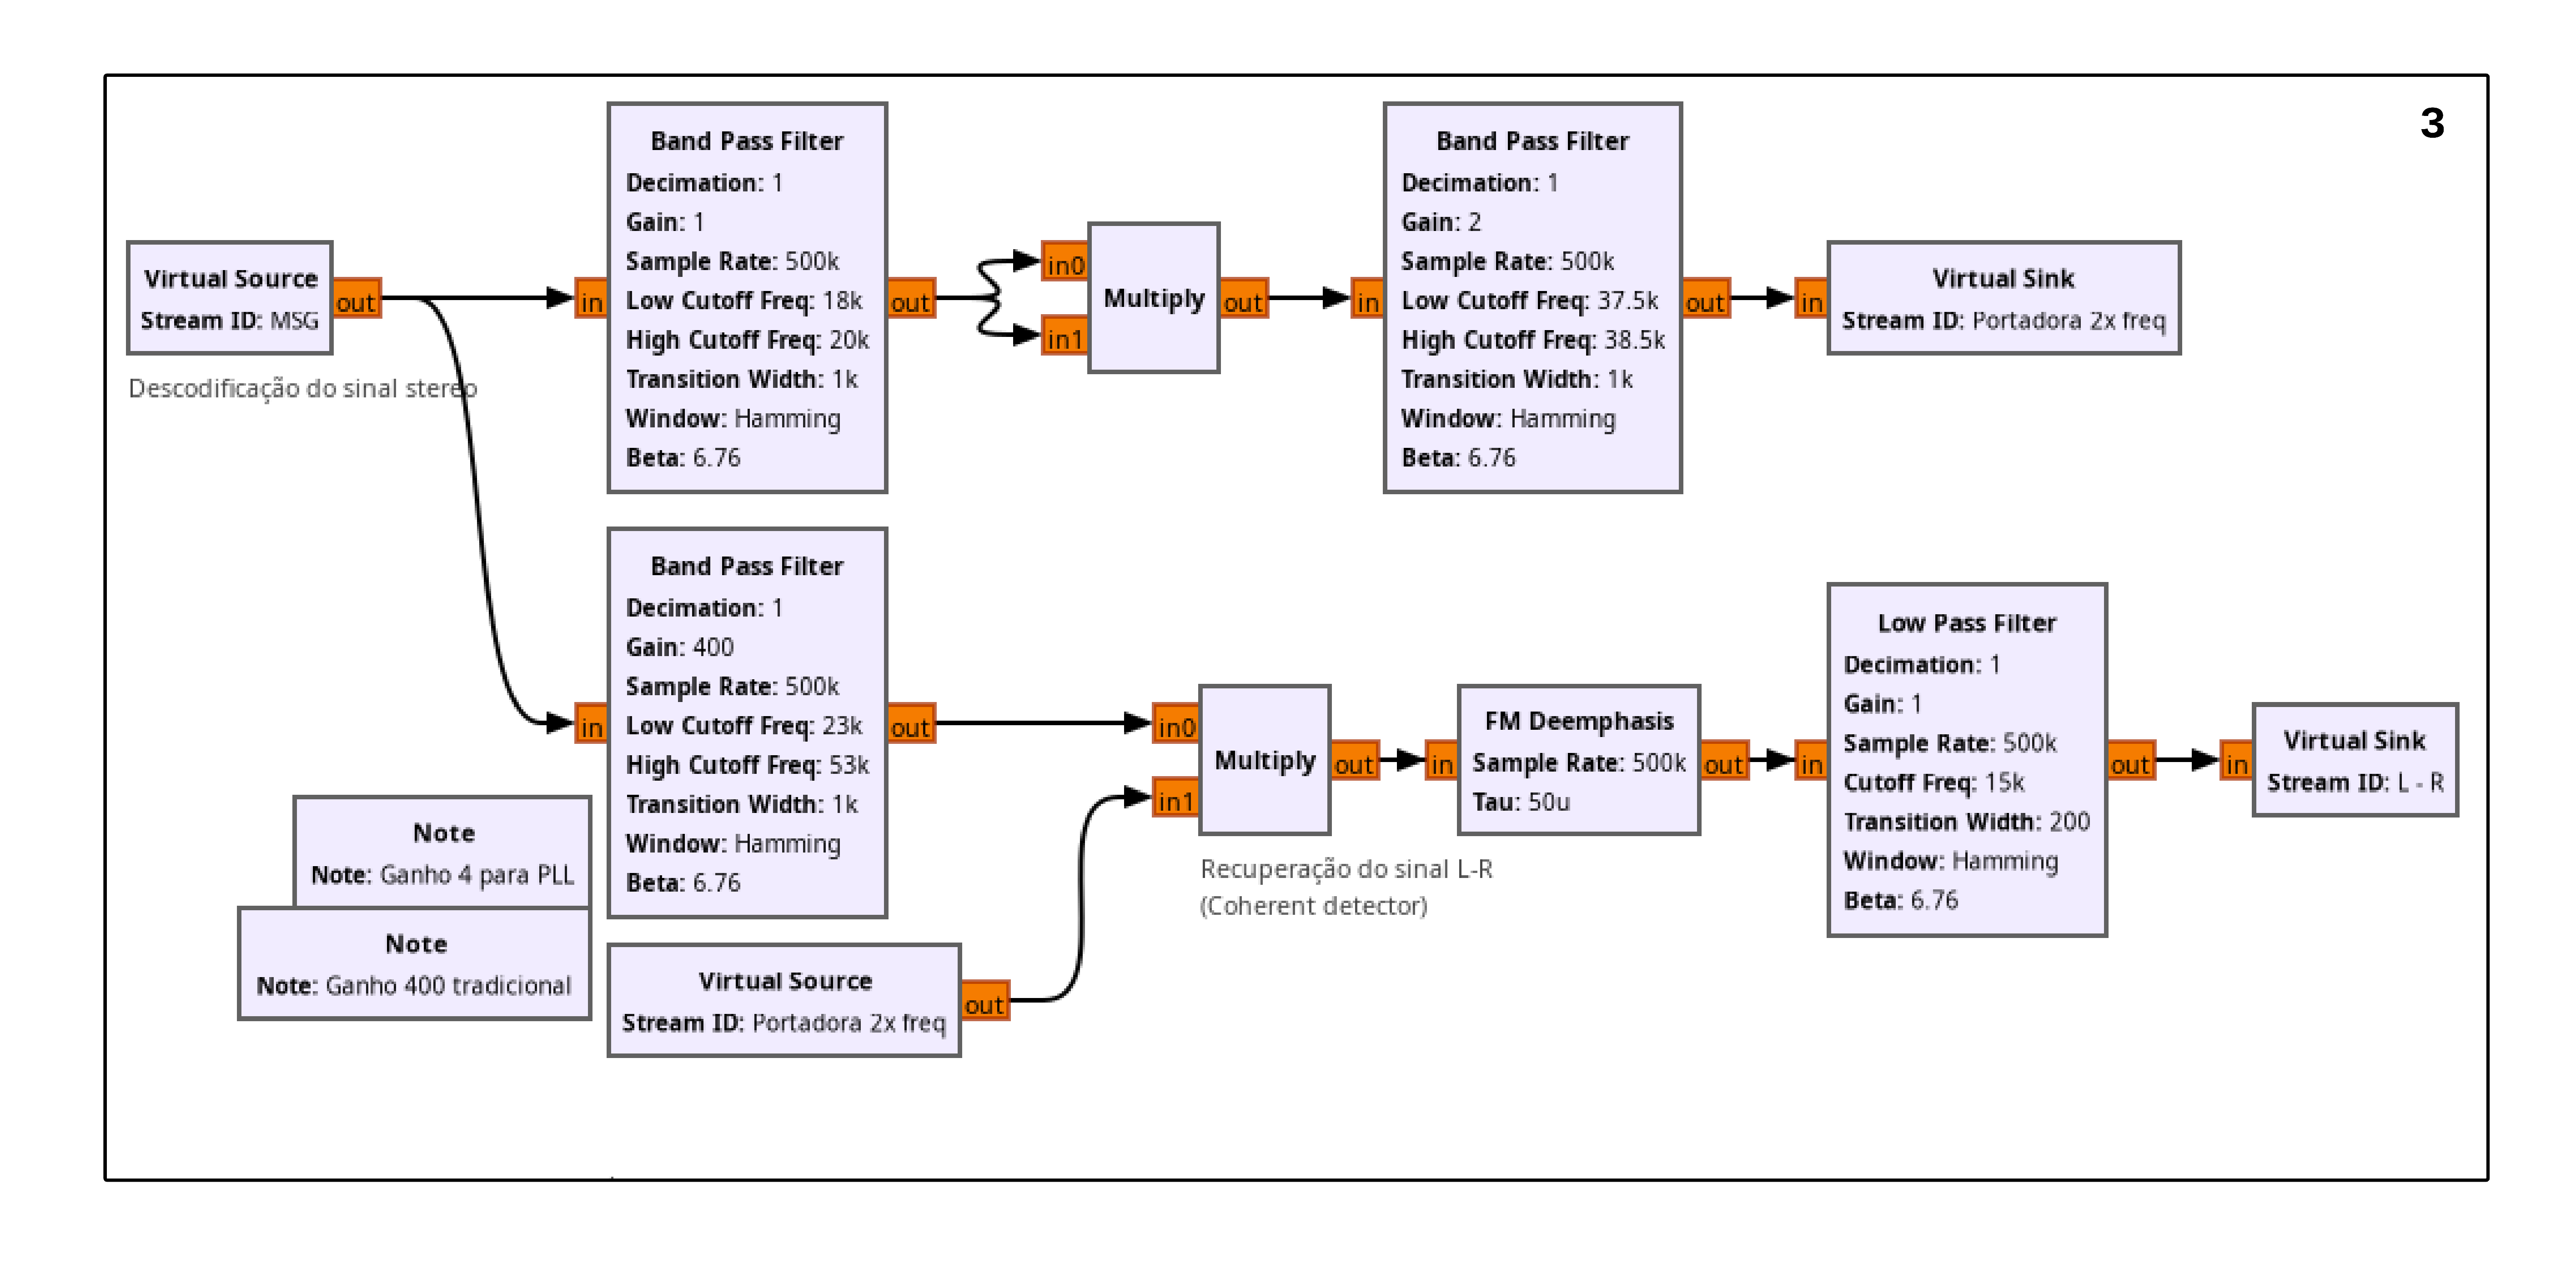
\includegraphics[width = \linewidth]{img/mods/modulo3.png}
    \caption{Recuperação da componente estereofónica da mensagem.}
    \label{fig:modulo3}
\end{figure}
%\fi

Este \hyperref[subsec:mod3]{módulo} pode ser visto em dois momentos: 
\begin{itemize}
    \item[$\mapsto$] \hyperref[subsubsec:regen]{Regeneração da subportadora e duplicação da sua frequência} \hyperref[fig:modulo3]{(no ramo superior)}
    \item[$\mapsto$] \hyperref[subsubsec:coherent]{Deteção coerente da DSB-SC $L-R$} \hyperref[fig:modulo3]{(no ramo inferior)}
\end{itemize}
%1
%1
%=============================--B--=============================%
\newpage
\subsubsection{1. Regeneração da subportadora e duplicação da sua frequência}
\label{subsubsec:regen}

A recuperação tradicional da portadora implica a passagem da mensagem por um filtro passa-banda muito fino (\textit{narrow-band}) em torno dos $19\ \text{kHz}$ (vide \hyperref[fig:stereo_spectrum]{Fig. 1}), para a recuperação da subportadora piloto. O posterior processo de duplicação de frequência envolve multiplicar este \textit{output} do filtro por si próprio:
$$\text{Narrow-band BPF $\sim$19 kHz} \implies \text{output :=}\ K \cdot\cos{(2\pi f_c\cdot t)} $$
$$ \text{Portadora 2x freq.}\ =  (K \cdot\cos{(2\pi f_c\cdot t)})^2 =$$
$$ = K^2 \cdot \cos^2{(2\pi f_c\cdot t)} = K^2 \cdot (\frac{1}{2} + \frac{1}{2}\cos{(2\pi (2f_c)\cdot t)})$$

É então aplicado um filtro passa-banda em volta dos $38\ \text{kHz}$, ou, teoricamente, um passa-alto\footnotemark[1], para a destruição da componente DC, com um ganho de 2 (dadas as identidades trigonométricas), e finalmente:
$$ \pmb{\therefore}  \text{\textbf{Portadora 2x freq.}} = K^2\cdot \cos{(2\pi (2f_c)\cdot t)}$$

\footnotetext[1]{No entanto, menos desejável nesta aplicação, já que o foco do passa-alto não é isolar a portadora do ruído, mas sim eliminar a componente estática.}
%2
%2
%=============================--C--=============================%
\subsubsection{2. Deteção coerente da DSB-SC $L-R$}
\label{subsubsec:coherent}

Voltando ao processo de recuperação do sinal $L-R$. Devemos primeiro analisar a \hyperref[fig:modulo3]{Fig. M3}, onde é aparente um ganho de 400 no filtro passa-banda (com frequências de corte de acordo com o espectro da mensagem já mencionado) que isola a componente estereofónica DSB-SC.

A dedução desta constante de correção foi efetuada através de uma análise teórica e prática:

Analisando somente o processo de deteção coerente, obtemos:
$$\text{DSB-SC L-R :=}\ [L-R]\cos{(2\pi (2f_c)\cdot t)}$$
$$\implies (\text{DSB-SC L-R})\cdot (\text{Portadora 2x freq.})=$$
$$= (\text{DSB-SC L-R})\cdot K^2 \cos{(2\pi (2f_c)\cdot t)} =$$
$$= [L-R]\cdot K^2\cos^2{(2\pi (2f_c)\cdot t)} =$$
$$= [L-R]\cdot K^2\left(\frac{1}{2} + \frac{1}{2}\cos{(2\pi (4f_c)\cdot t)}\right) $$

Que após a passagem no filtro passa-baixo final (assumindo ganho unitário em todos os filtros deste ramo, para demonstrar os fatores a compensar):
$$\therefore \text{Sinal $[L-R]$ recuperado por compensar}\ = [L-R]\cdot \frac{K^2}{2}$$

No entanto a prova empírica (exercida com os ficheiros de calibração LEFT e RIGHT) indica que é necessária a correção de um fator multiplicativo extra de 1/2 para que os sinais $L+R$ e $L-R$ possuam a mesma amplitude, de modo a que seja possível proceder ao \hyperref[subsec:mod4]{módulo seguinte} e efetuar a recuperação de $L$ e $R$ de forma bem sucedida.

\newpage

\begin{figure}[ht] 
    \begin{subfigure}[b]{0.5\linewidth}
        \centering
        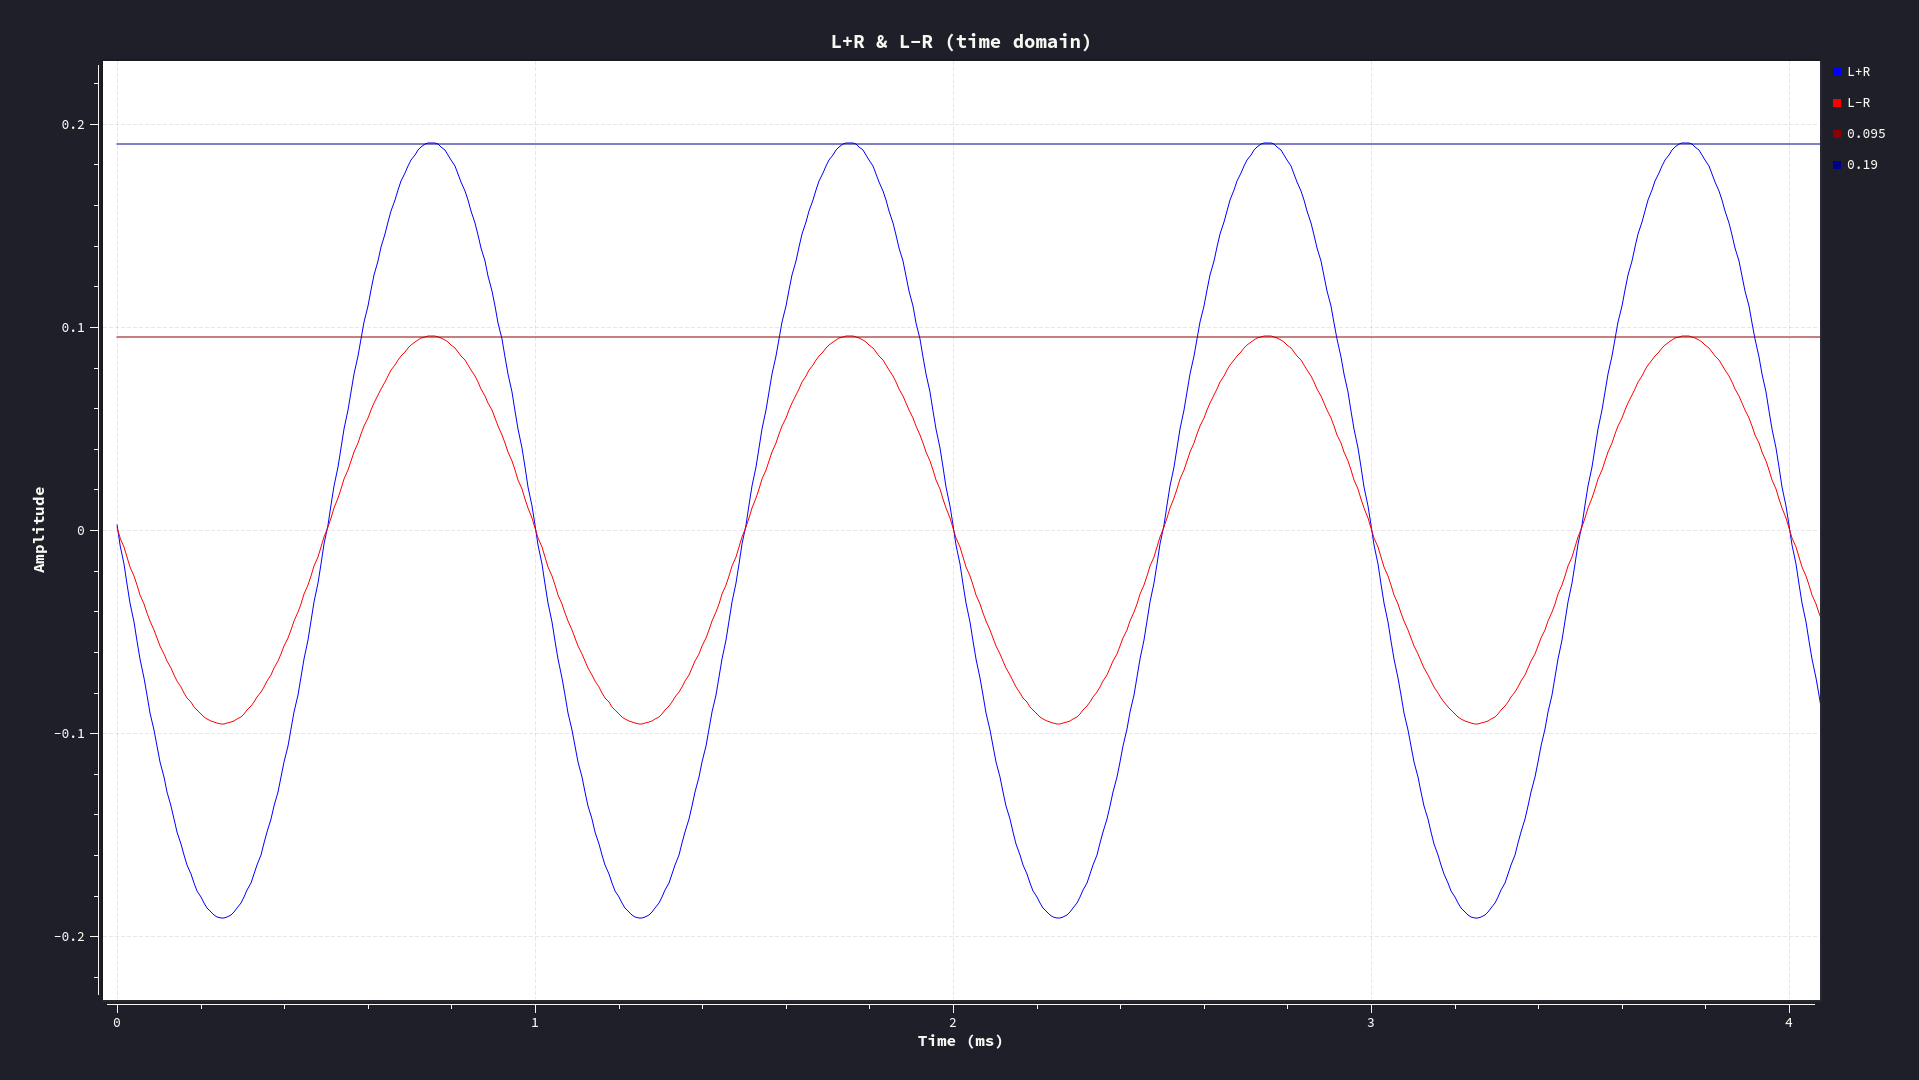
\includegraphics[width=0.8\linewidth]{img/1_2LEFT.png}
        \caption{LEFT: visualização de $L+R$ e $L-R$ (domínio \\ do tempo)} 
        \label{fig:aaa} 
        \vspace{1ex}
    \end{subfigure}%% 
    \begin{subfigure}[b]{0.5\linewidth}
        \centering
        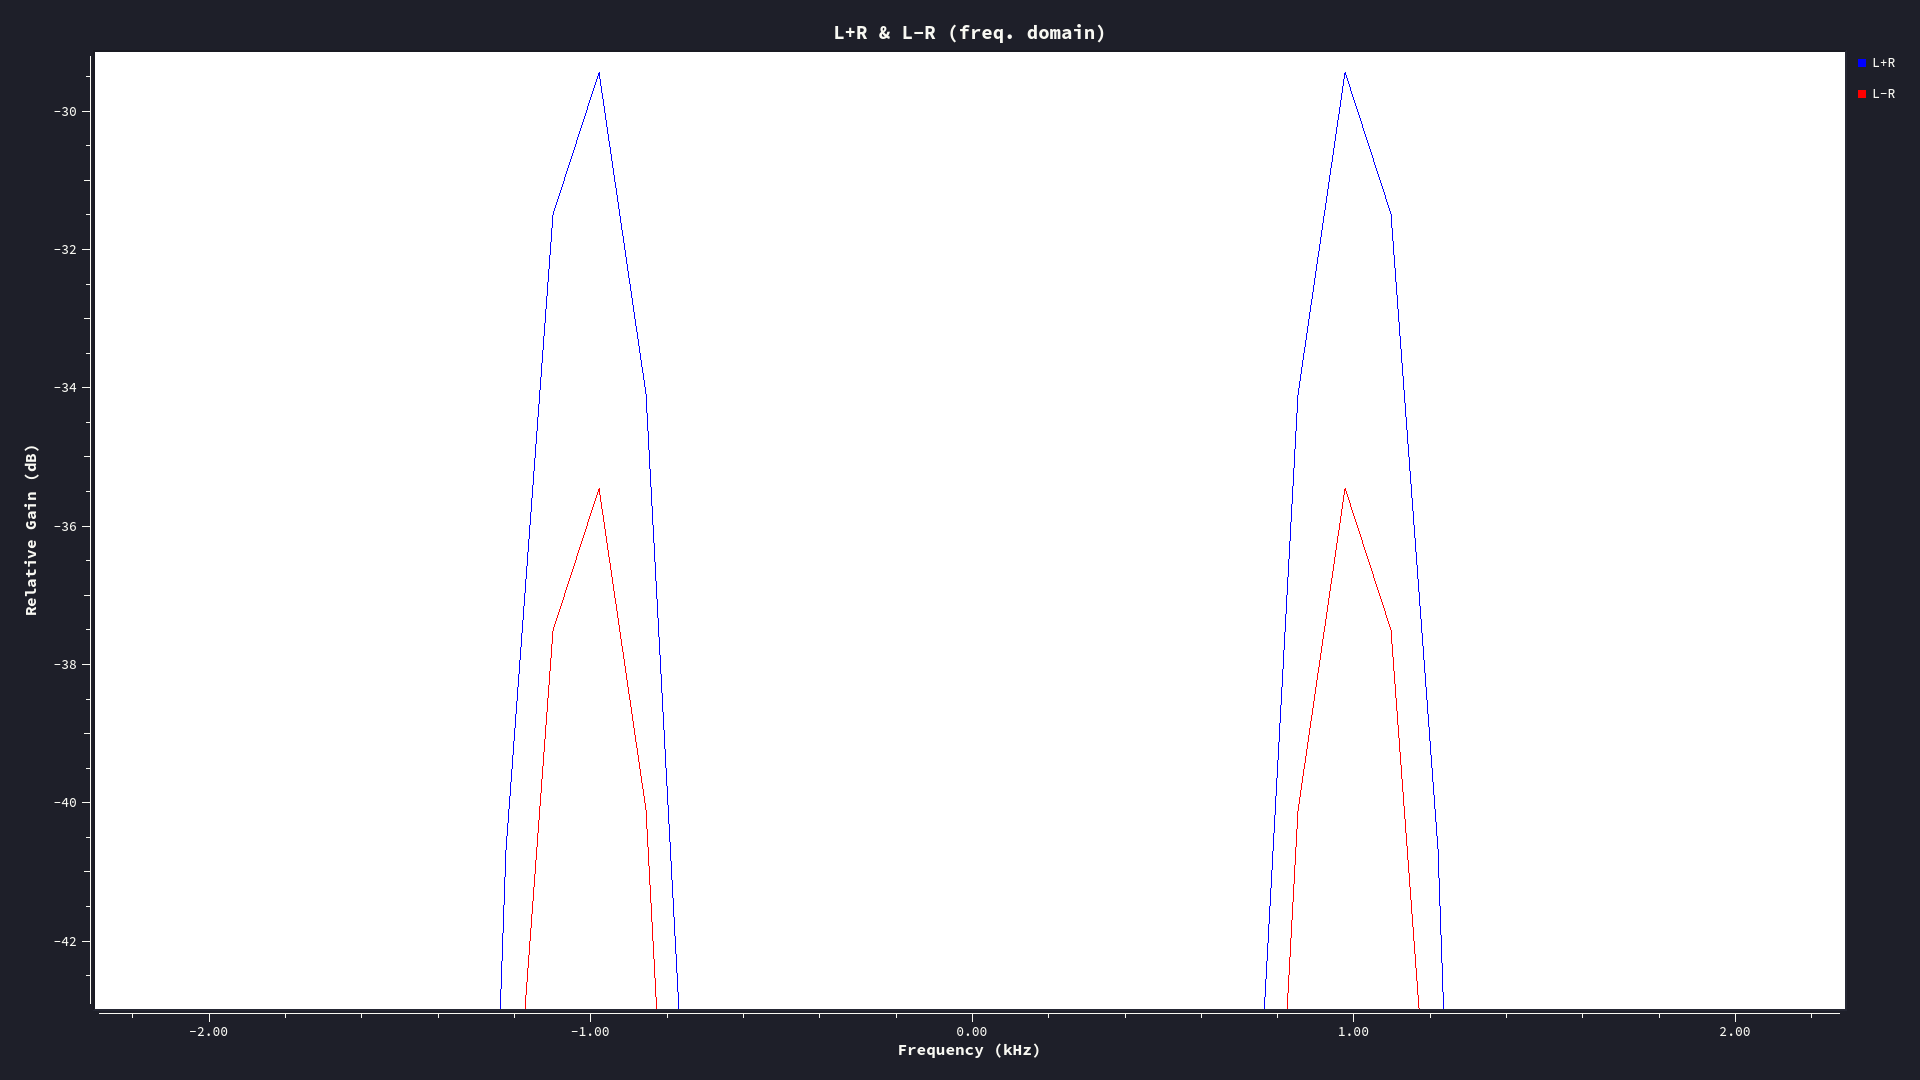
\includegraphics[width=0.8\linewidth]{img/1_2LEFTdB.png} 
        \caption{LEFT: visualização de $L+R$ e $L-R$ (domínio \\ da frequência)} 
        \label{fig:bbb} 
        \vspace{1ex}
    \end{subfigure} 
    \begin{subfigure}[b]{0.5\linewidth}
        \centering
        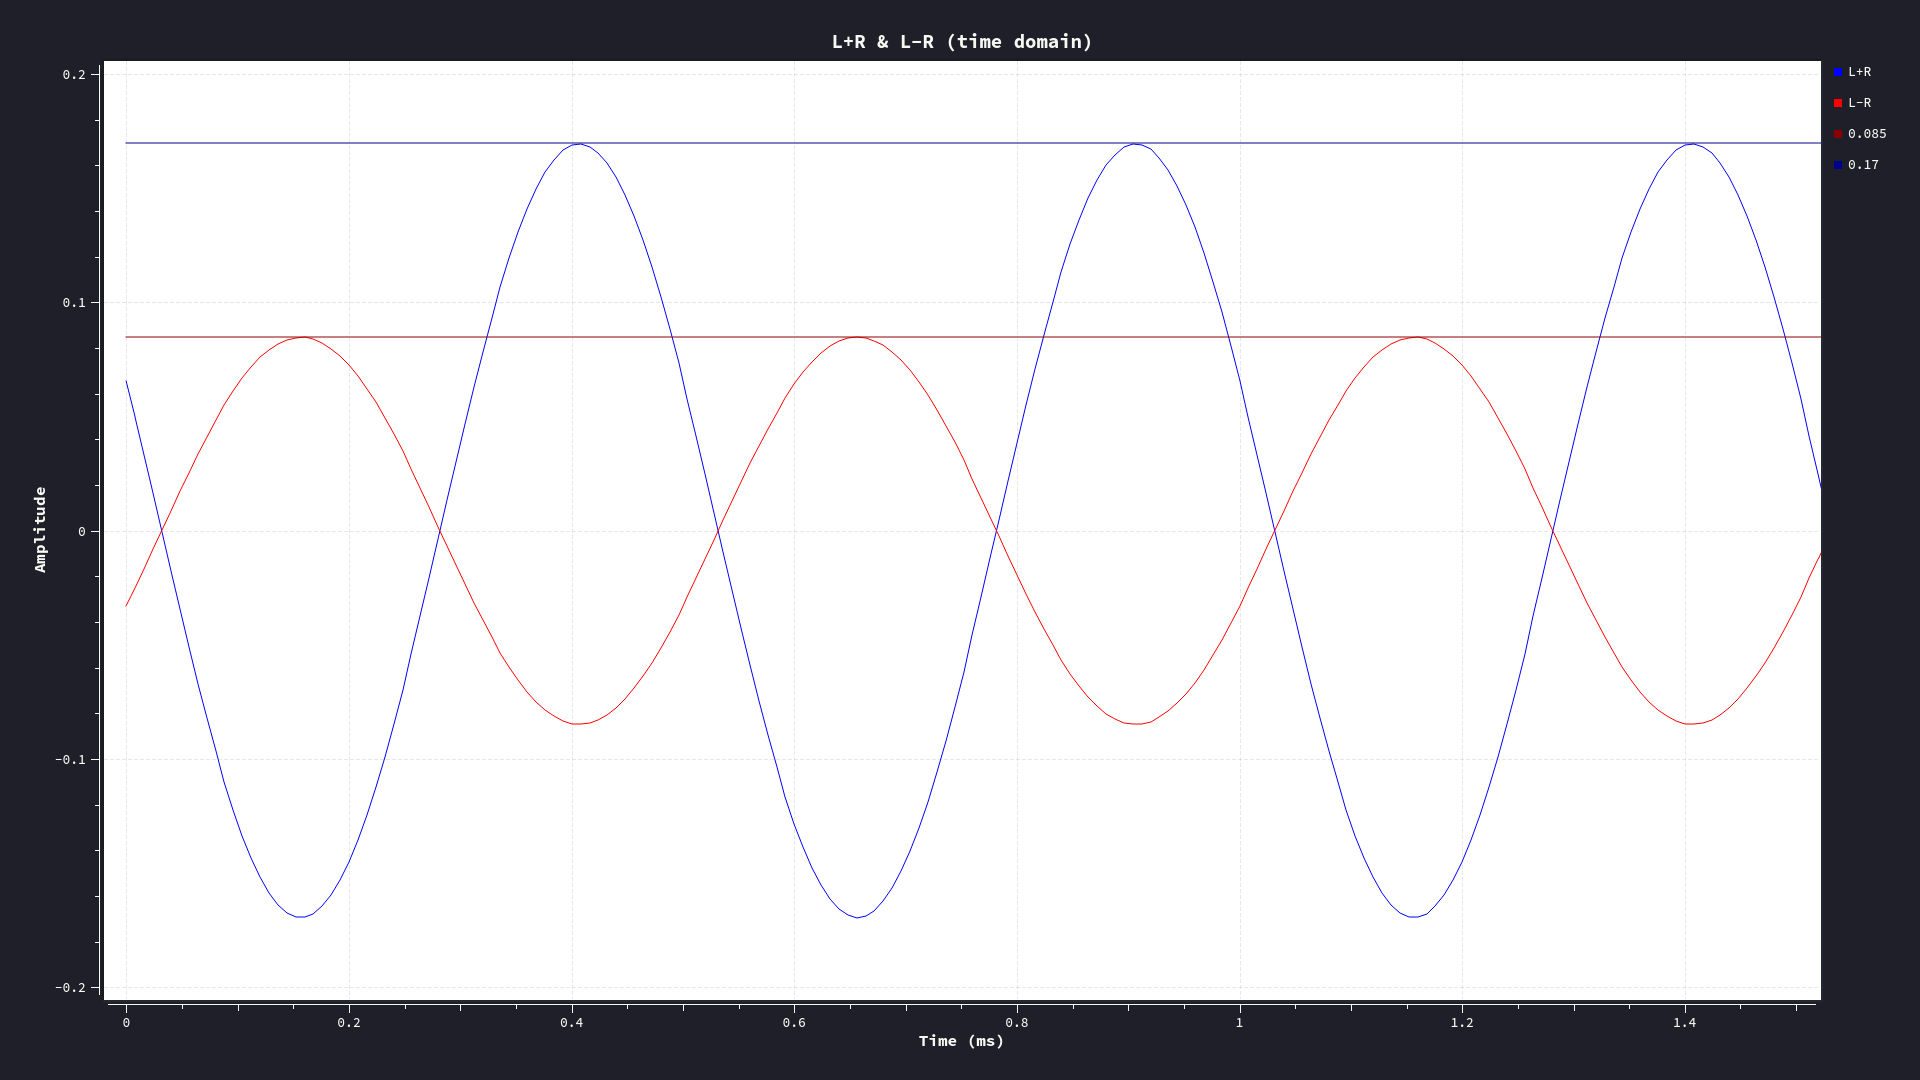
\includegraphics[width=0.8\linewidth]{img/1_2RIGHT.png}
        \caption{RIGHT: visualização de $L+R$ e $L-R$ (domínio \\ do tempo)} 
        \label{fig:ccc} 
        %%\vspace{4ex}
    \end{subfigure}%% 
    \begin{subfigure}[b]{0.5\linewidth}
        \centering
        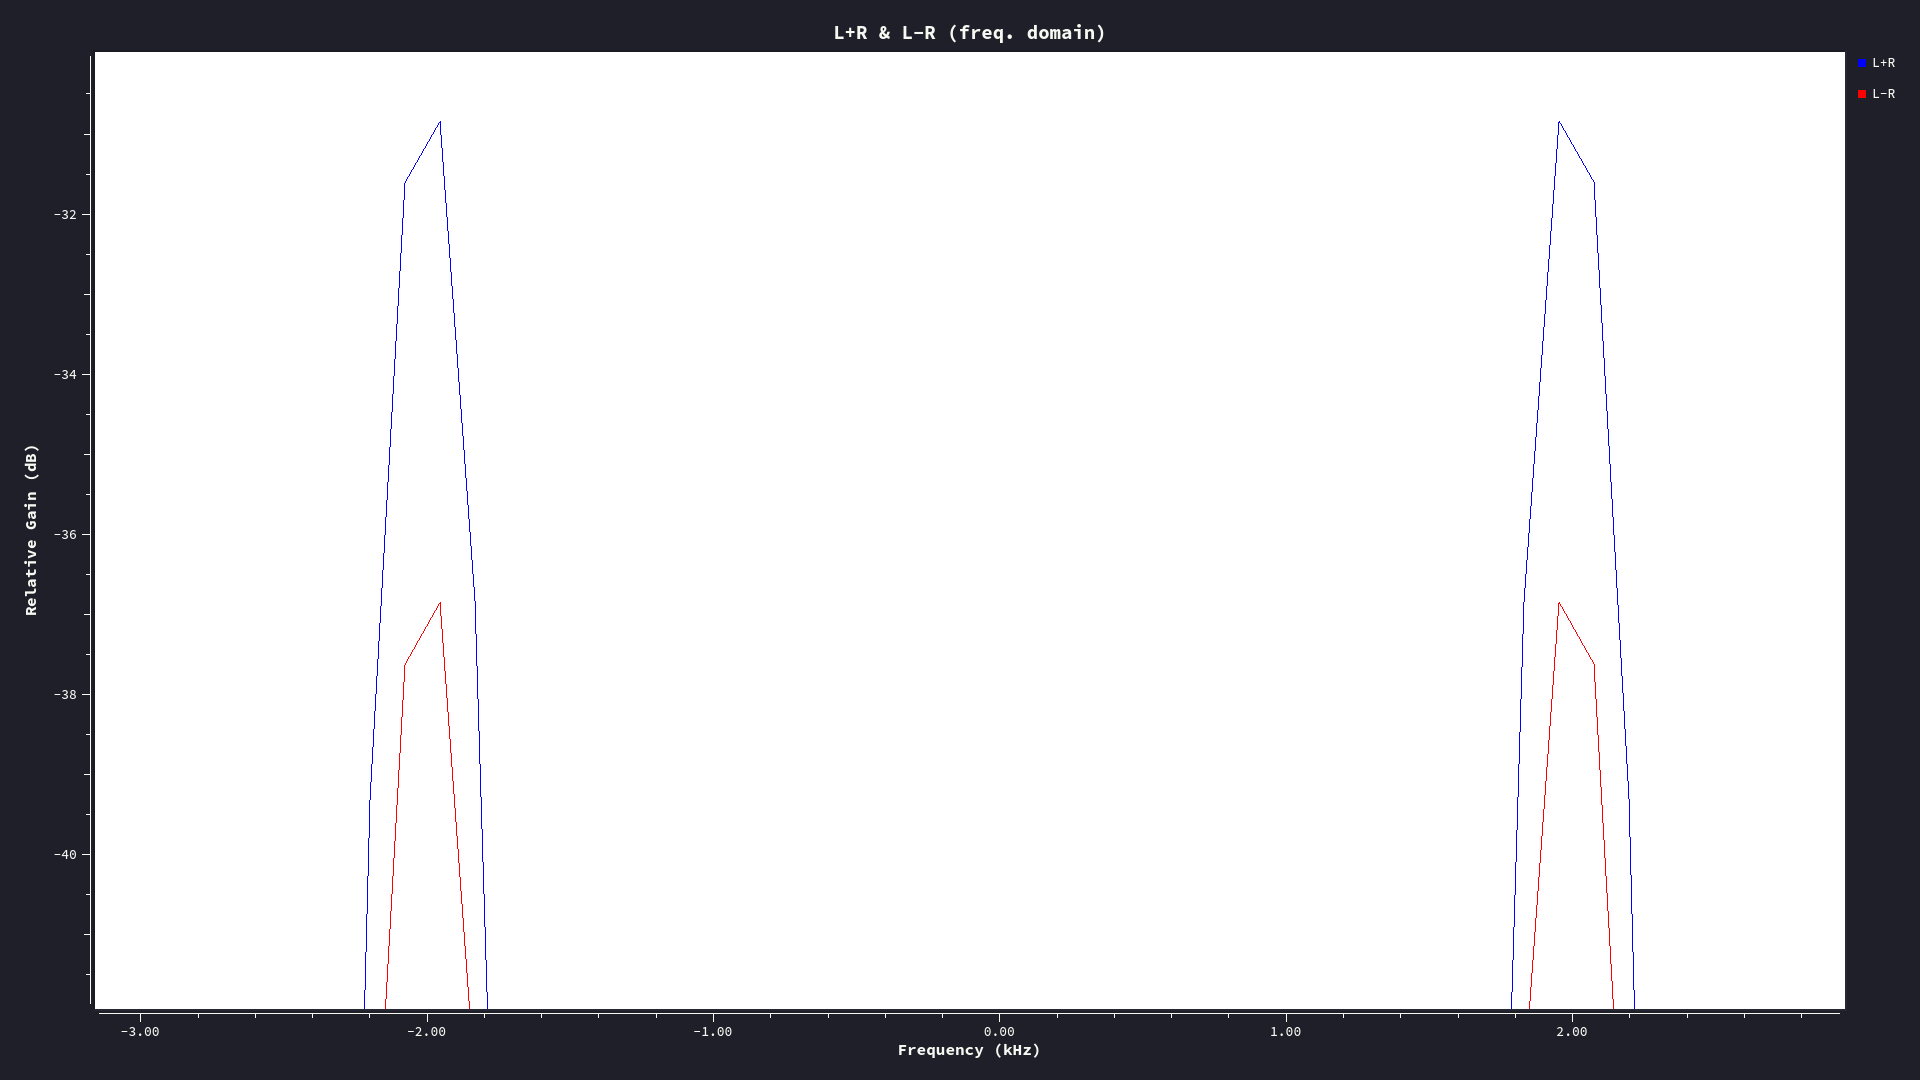
\includegraphics[width=0.8\linewidth]{img/1_2RIGHTdB.png} 
        \caption{RIGHT: visualização de $L+R$ e $L-R$ (domínio \\ da frequência)} 
        \label{fig:ddd} 
        %%\vspace{4ex}
    \end{subfigure} 
    \caption{Visualização do fator de 1/2 extra a compensar.}
    \label{fig:multiplas3}
\end{figure}

Verificando a \hyperref[fig:stereo_spectrum]{Fig. 1}, é aparente que a componente estereofónica DSB-SC dispõe metade do nível de modulação da componente monofónica em cada uma das bandas\cite{transmission_standards_for_fm_sound_broadcasting_at_vhf}. Isto é traduzido nos resultados observados na \hyperref[fig:multiplas3]{Fig. M4}, i.e., no domínio do tempo a componente $L-R$ tem exatamente metade da amplitude de $L+R$, e no domínio da frequência o pico de $L-R$ situa-se a cerca de $6$ dB a baixo\footnotemark[2] do de $L+R$.

\footnotetext[2]{C.A.: $-6$ dB $= 10^{-6/20} \approx 0.5$}

O mesmo raciocínio é aplicado para a obtenção do fator $K$ mencionado anteriormente. 

\begin{figure}[H]
    \centering
    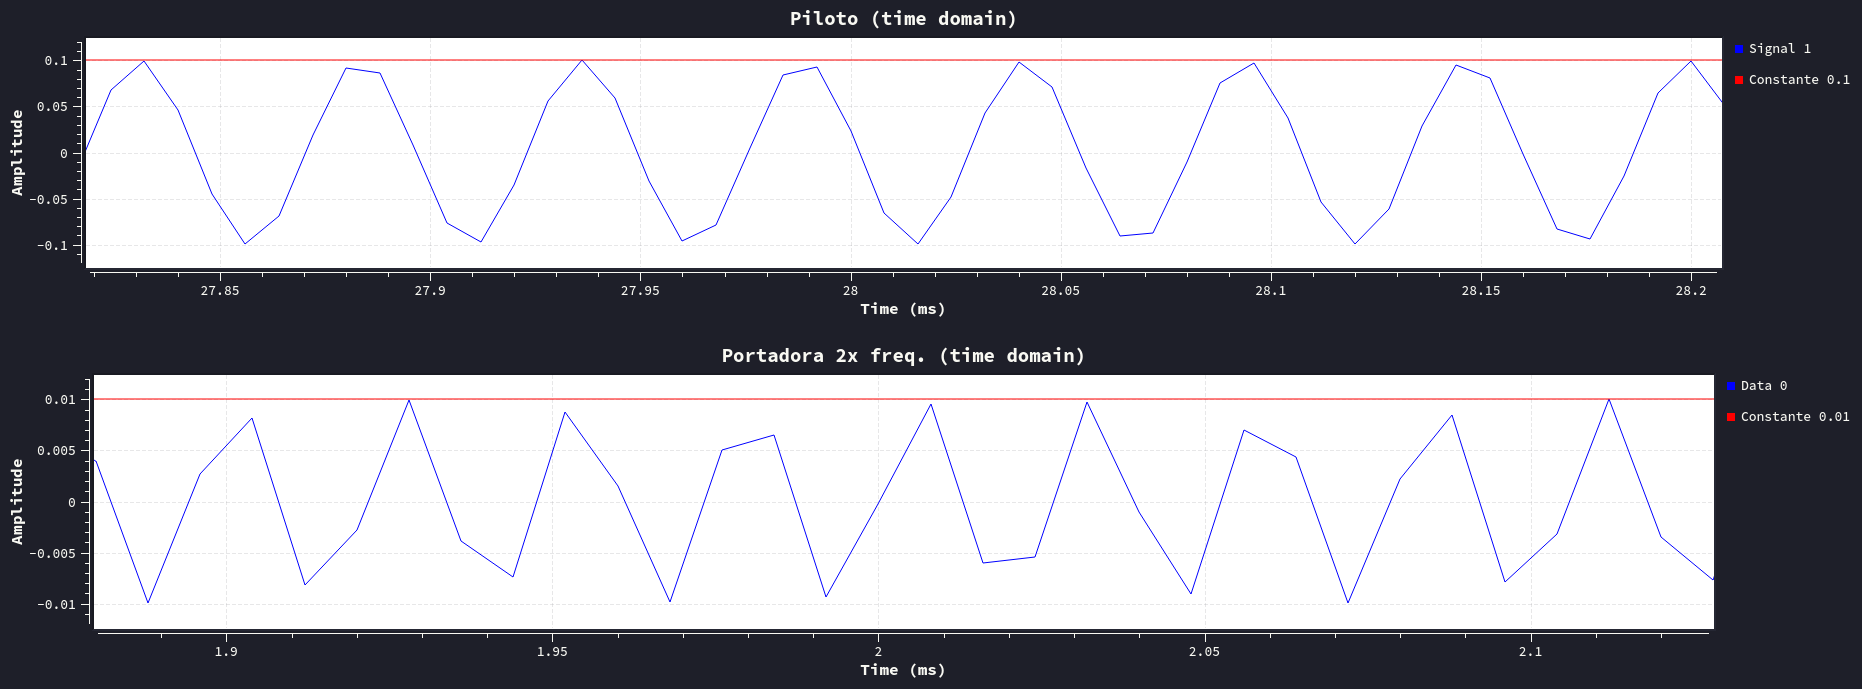
\includegraphics[width = 0.6\linewidth]{img/constanteK.png}
    \caption{Representação no domínio temporal da portadora regenerada (com amplitude $K$) e da respetiva portadora com o dobro da frequência após o processo de duplicação (com aplitude $K^2$).}
    \label{fig:constanteK}
\end{figure}
Deste modo, $K = 0.1$.
$$ \pmb{\therefore} \text{\textbf{Fator total a compensar}}\ = \frac{1}{2}\cdot\frac{1}{2}\cdot 0.01 = \frac{1}{400} \implies \text{\textbf{Ganho}}\ = 400$$

Após estas correções, o sinal $L-R$ está de acordo para o processamento correto\footnotemark[3] no \hyperref[subsec:mod4]{módulo que se sucede}.

\footnotetext[3]{É admitido que os ficheiros de calibração nos traduziram o correto fator de compensação deste ramo para a desmultiplexação de qualquer sinal neste formato. Dado que as emissoras rádio em Lisboa transmitem em formato stereo, mas, maioritariamente com $L=R$, não foi possível realizar mais ensaios que garantissem a robustez deste resultado, visto que dipõem $L-R=0$ efetivamente.}
%=============================--A--=============================%
\subsection{Módulo 4 $\pmb \mapsto$ \textit{Dematrixing} e reprodução sonóra de $L$ e $R$}
\label{subsec:mod4}

%\iffalse
\begin{figure}[H]
    \centering
    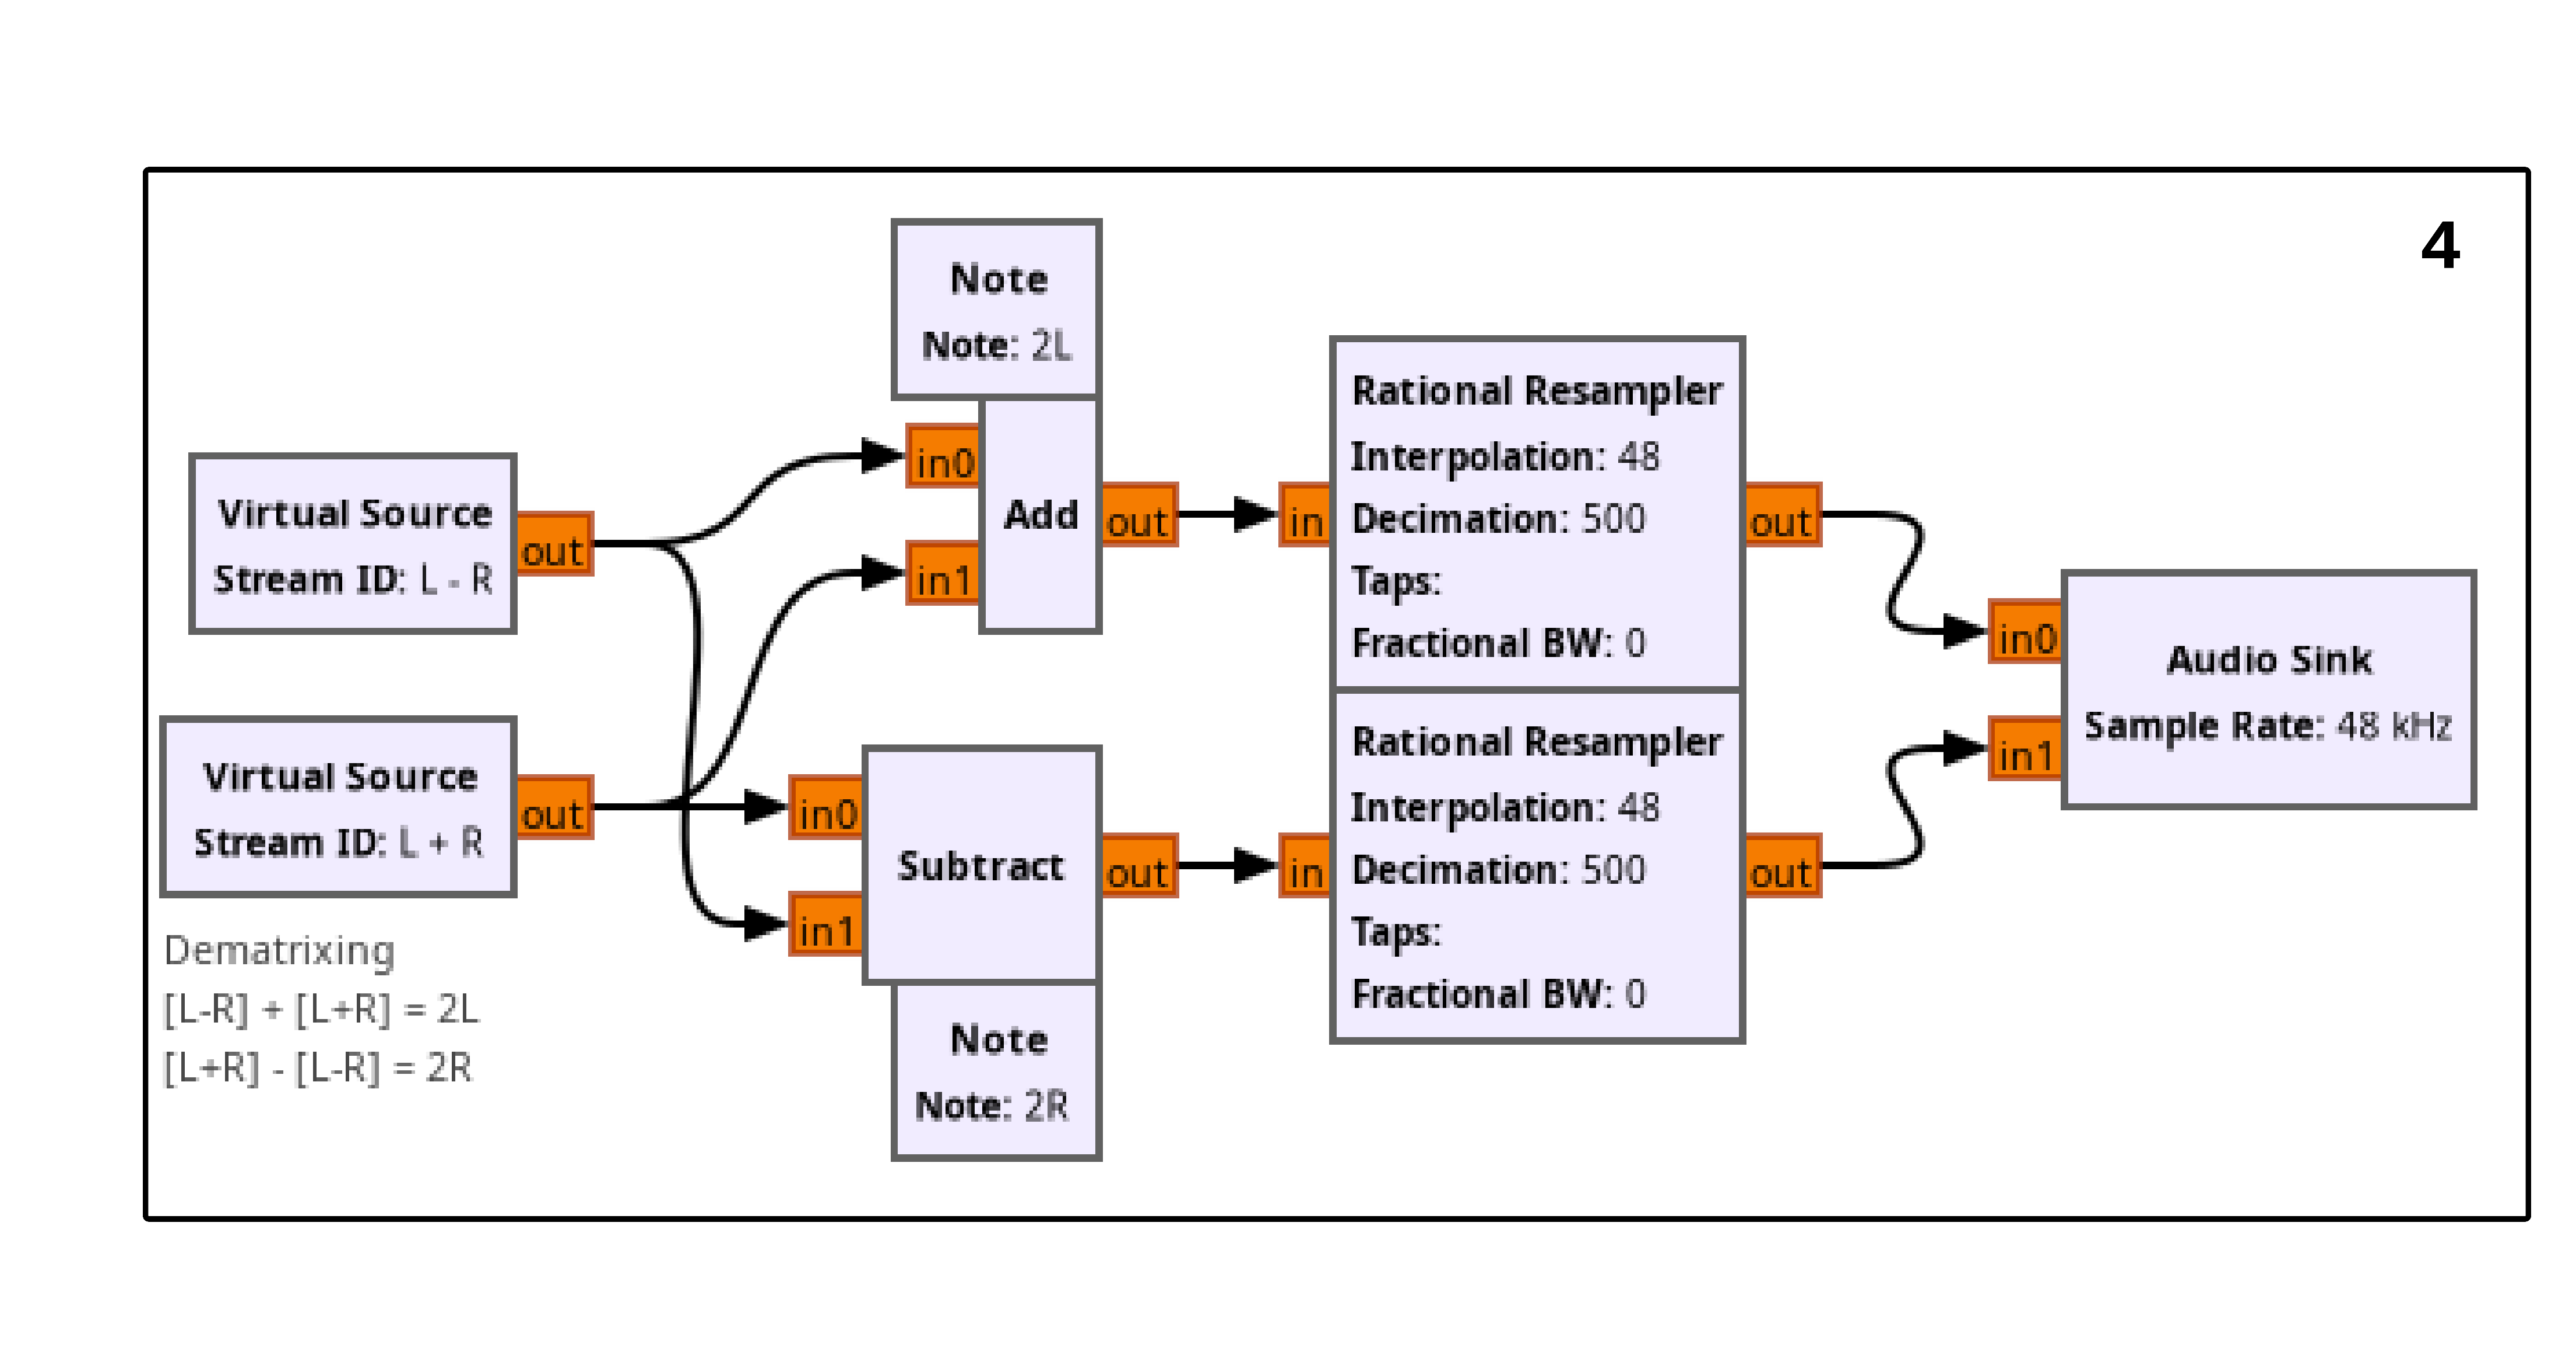
\includegraphics[width = 0.6\linewidth]{img/mods/modulo4.png}
    \caption{Recuperação dos sinais $L$ e $R$ através do processo de \textit{dematrixing}.}
    \label{fig:modulo4}
\end{figure}
%\fi

Por fim, tal como referido na introdução, a recuperação das componentes associadas ao ouvido esquerdo ($L$) e direito ($R$) do sinal é bastante trivial. Aplicando o processo de \textit{dematrixing} a $m_1(t)$ e $m_2(t)$, com auxilio dos blocos de "Add" e "Subtract" obtemos:

\begin{equation*}
  \left\{\begin{array}{@{}l@{}}
    m_1(t)+m_2(t)=2L\\
    m_1(t)-m_2(t)=2R
  \end{array}\right.\,
\end{equation*}

Contudo, é importante reparar que após este processo é essencial reduzir o ritmo amostral para $48$ kHz antes da ligação ao "Audio Sink" (reprodução do sinal de áudio). Este processo é assegurado, tal como descrito no guia, pelo bloco "Rational Resampler" em adequação com as características da placa de som do computador.
    %% biblio/webgraphy
    \clearpage
    \bibliographystyle{unsrtnat}
    \nocite{*}
    {\footnotesize
    \bibliography{refs}}
    %% attachments
    \newpage
    \renewcommand{\thefigure}{A\arabic{figure}}
\renewcommand{\thetable}{A\arabic{table}}
\setcounter{figure}{0}
\section{Apêndice}
\subsection{Regeneração da portadora com PLL}
\label{subsec:PLL}

%\iffalse
\begin{figure}[H]
    \centering
    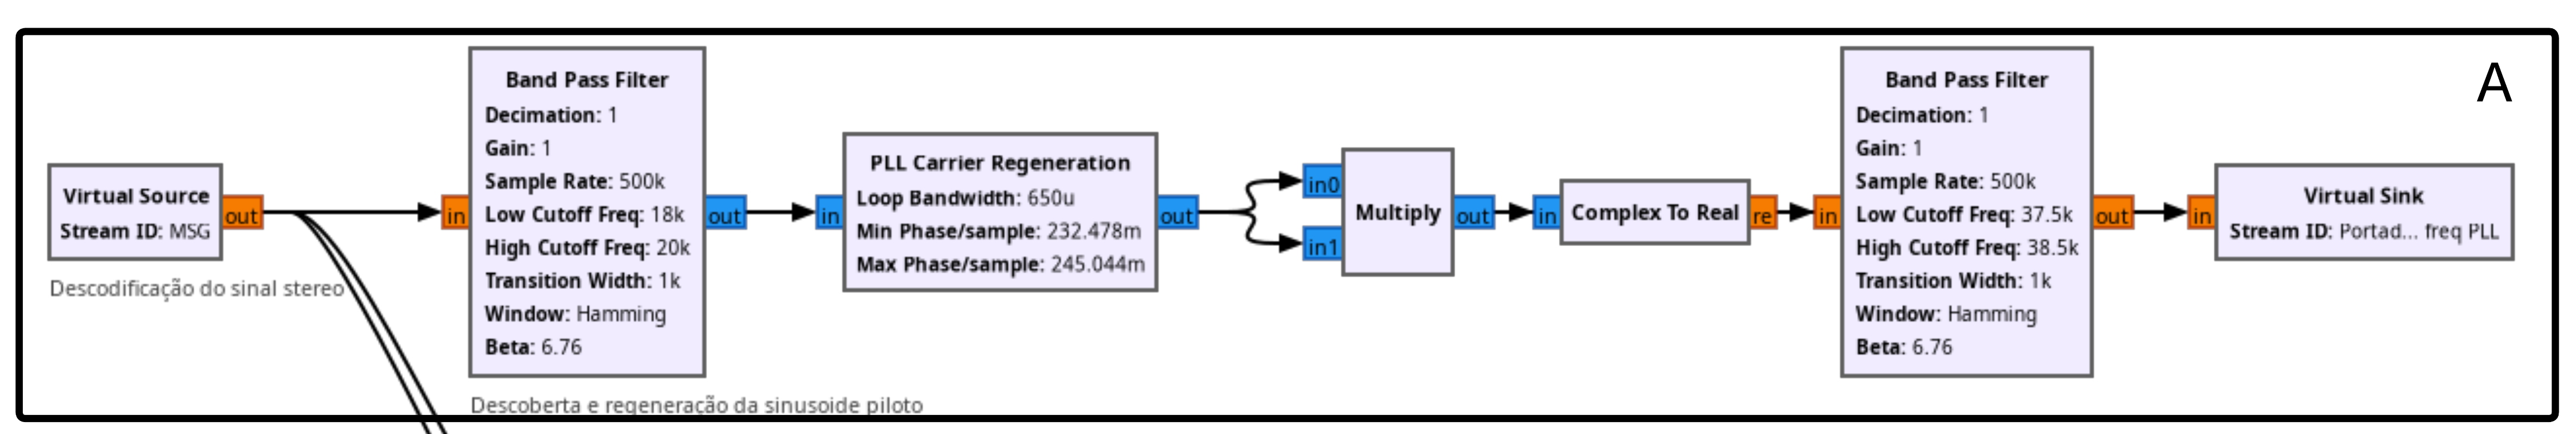
\includegraphics[width = 0.9\linewidth]{img/appendix/PLL_galore.png}
    \caption{Esquema de regeneração da portadora e duplicação de frequência com o PLL.}
    \label{fig:appendix0}
\end{figure}
%\fi

O processo de regeneração da portadora, analisado no \hyperref[subsec:mod3]{módulo 3}, pode ser efetuado com o auxilio de um bloco \textit{"PLL Carrier Regeneration"}. A seguinte \hyperref[fig:appendix1]{Fig. A2} ilustra o funcionamento genérico de um PLL. 
\vspace{0.5em}
\iffalse
\begin{figure}[H]
    \centering
    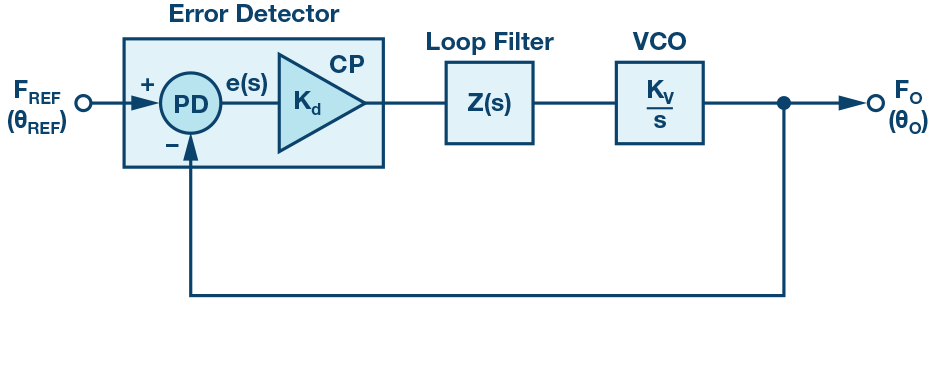
\includegraphics[width = 0.55\linewidth]{img/appendix/PLL.png}
    \caption{Configuração genérica do PLL.}
    \label{fig:appendix1}
\end{figure}
\fi

\begin{tabular}{C{8cm}  L{6.5 cm}}
        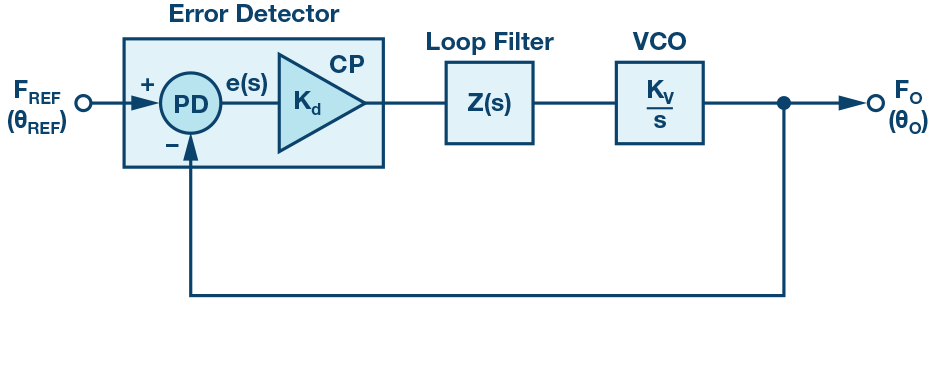
\includegraphics[width=\linewidth]{img/appendix/PLL.png}\captionof{figure}{Configuração genérica do PLL\cite{person}.} & 
        Dado que ultrapassa o âmbito da UC, procedemos apenas a uma análise empírica do bloco supramencionado que: \textit{"(...) locks onto a [possibly noisy] reference carrier on the input and outputs a clean version which is phase and frequency aligned to it."}\cite{pll_ref_out-gnuradio}
    \end{tabular}
    
\vspace{0.5em}
\noindent\fcolorbox{black}{white}{%
    \minipage[t]{\dimexpr\linewidth-2\fboxsep-2\fboxrule\relax}
        \textbf{Observação 1} $\rightarrow$ Após uma análise espectral da portadora regenerada, verificou-se, de facto, uma versão mais limpa do sinal de entrada, que nos é favorável dado que pretendemos eliminar ao máximo o ruído nos sinais auxiliares na descodificação da mensagem. No entanto, o fator $K$ da subportadora piloto perde-se neste processo e a portadora que sai do PLL dispõe de uma amplitude unitária.
    \endminipage}
\newline\break
\noindent\fcolorbox{black}{white}{%
    \minipage[t]{\dimexpr\linewidth-2\fboxsep-2\fboxrule\relax}
        \textbf{Observação 2} $\rightarrow$ Visto que uma emissora de sinal FM em Lisboa, tipicamente não transmite conteúdo stereo (i.e., o sinal tem tipicamente formato stereo, mas o conteúdo da esquerda é equivalente ao da direita, $L=R$), o facto da amplitude da portadora regenerada ser unitário acaba por comprometer a qualidade sonora audível, dado que eleva o ruído de fundo proveniente da fase de deteção coerente da componente $L-R$ (que deveria ser nula teoricamente, mas apresenta-se como uma camada de ruído). 
    \endminipage}
\newline\break
Devido a estas duas observações, foi decidido não apresentar esta solução como principal, visto que compromete a qualidade sonora audível. No entanto, é importante porque salienta a existência de outros métodos de recuperação da portadora, e passando à citação:

\textit{"(...) PLL chips now relatively cheap, (...) PLL applications enables high quality audio to be demodulated from an FM signal."}\cite{notes}

\end{document}
